\documentclass[12pt]{report}

% includes
\usepackage{geometry}           % page size
\usepackage[utf8]{inputenc}     % encoding
\usepackage{palatino}           % font
\usepackage[romanian]{babel}    % language
\usepackage{graphicx}           % images
\usepackage{indentfirst}        % indentation
\usepackage[nottoc]{tocbibind}  % table of contents style
\usepackage[unicode]{hyperref}  % references from the table of contents
\usepackage{float}
\usepackage[export]{adjustbox}

% includes options
\geometry{  a4paper,            % scientific thesis standard
            left=3cm,
            right=2cm,
            top=2cm,
            bottom=2cm,
 }
\graphicspath{{images/}}        % path where the images are located
\setlength{\parindent}{1cm}     % paragraph indentation

%& -job-name=2022_Licenta_Dascalu_Andrei
% other options
\linespread{1.5}                % space between lines
\renewcommand*\contentsname{Cuprins}    % table of contents name

% the document content
\begin{document}
    % macros (global)
    \newcommand{\university}    {Universitatea "Alexandru-Ioan Cuza" din Iași}
\newcommand{\universityg}   {Universității "Alexandru-Ioan Cuza" din Iași} % genitive
\newcommand{\faculty}       {Facultatea de informatică}
\newcommand{\facultyg}      {Facultății de informatică} % genitive
\newcommand{\speciality}    {informatică}
\newcommand{\promotion}     {2022}                                  %<---------

\newcommand{\thesistype}    {Lucrare de licență}
\newcommand{\thesistitle}   {Bachelor Thesis Distributor}    %<---------
\newcommand{\thesissubtitle}   {Aplicație de repartizare a studenților la profesori coordonatori de licență}    %<---------


\newcommand{\authorlast}    {Dascălu}                               %<---------
\newcommand{\authorfirst}   {Andrei}
\newcommand{\authornamefl}  {\authorfirst \space \authorlast} % first name first
\newcommand{\authornamelf}  {\authorlast \space \authorfirst} % last name first
\newcommand{\authorbirth}   {03 noiembrie 2000}                      %<---------
\newcommand{\authoraddress} {România, jud. Iași, mun. Iași, strada Sf. Teodor nr. 14} %<---------
\newcommand{\authorcnp}     {5001103226752}                         %<---------

\newcommand{\session}       {*iunie, 2022}                       %<---------
\newcommand{\coordinator}   {Lect. Dr. Frăsinaru Cristian}               %<---------

\newcommand{\dottedline}    {............................}
    
    % front-matter
    \pagenumbering{gobble}
    
    % define the cover page
\begin{titlepage}
    \begin{center}
        % the university and faculty
        \large
        \MakeUppercase{\university}
        
        \LARGE
        \textbf{\MakeUppercase{\faculty}}
        
        % the faculty logo
        \vspace{1cm}
        
\includegraphics[width=0.3\textwidth]{logoFii.png}
        
        % thesis title
        \vspace{1cm}
        \Large
        \MakeUppercase{\thesistype}
        
        \vspace{0.5cm}
        \LARGE
        \textbf{\thesistitle}
        
        \thesissubtitle
        
        % author
        \vspace{2cm}
        \Large
        propusă de
        
        \vspace{0.5cm}
        \LARGE
        \textbf{\authornamefl}
        
        % session
        \vfill
        \Large
        \textbf{Sesiunea:} \session
        
        % scientific coordinator
        \vspace{2cm}
        \Large
        Coordonator științific
        
        \vspace{0.5cm}
        \LARGE
        \textbf{\coordinator}
    \end{center}
\end{titlepage}
    % define the title page
\begin{titlepage}
    \begin{center}
        % the university and faculty
        \large
        \MakeUppercase{\university}
        
        \LARGE
        \textbf{\MakeUppercase{\faculty}}
        
        % thesis title
        \vspace{8cm}
        \huge
        \textbf{\thesistitle}
        
        % author
        \vspace{2cm}
        \LARGE
        \textbf{\authornamefl}
        
        % session
        \vfill
        \Large
        \textbf{Sesiunea:} \session
        
        % scientific coordinator
        \vspace{4cm}
        \Large
        Coordonator științific
        
        \vspace{0.5cm}
        \LARGE
        \textbf{\coordinator}
    \end{center}
\end{titlepage}
    \vspace*{\fill}

\begin{flushright}
    Avizat, \\
    Îndrumător lucrare de licență, \\
    \coordinator. \\
    Data: \dottedline \hspace{1cm} Semnătura: \dottedline
\end{flushright}

\vspace{1cm}
\begin{center}
    \large
    \textbf{Declarație privind originalitatea conținutului lucrării de licență}
\end{center}

Subsemnatul \textbf{\authornamelf} domiciliat în \textbf{\authoraddress}, născut la data de \textbf{\authorbirth}, identificat prin CNP \textbf{\authorcnp}, absolvent al \facultyg, \textbf{\faculty} specializarea \textbf{\speciality}, promoția \promotion, declar pe propria răspundere cunoscând consecințele falsului în declarații în sensul art. 326 din Noul Cod Penal și dispozițiile Legii Educației Naționale nr. 1/2011 art. 143 al. 4 și 5 referitoare la plagiat, că lucrarea de licență cu titlul \textbf{\thesistitle} elaborată sub îndrumarea domnului \textbf{\coordinator}, pe care urmează să o susțin în fața comisiei este originală, îmi aparține și îmi asum conținutul său în întregime.

De asemenea, declar că sunt de acord ca lucrarea mea de licență să fie verificată prin orice modalitate legală pentru confirmarea originalității, consimțind inclusiv la introducerea conținutului ei într-o bază de date în acest scop.

Am luat la cunoștință despre faptul că este interzisă comercializarea de lucrări științifice în vederea facilitării falsificării de către cumpărător a calității de autor al unei lucrări de licență, de diplomă sau de disertație și în acest sens, declar pe proprie răspundere că lucrarea de față nu a fost copiată ci reprezintă rodul cercetării pe care am întreprins-o.

\begin{flushright}
    Data: \dottedline \hspace{6cm} Semnătura: \dottedline
\end{flushright}

\vspace*{\fill}
\pagebreak
    \vspace*{\fill}
\begin{center}
    \large
    \textbf{Declarație de consimțământ}
\end{center}

Prin prezenta declar că sunt de acord ca lucrarea de licență cu titlul \textbf{\thesistitle}, codul sursă al programelor și celelalte conținuturi (grafice, multimedia, date de test, etc.) care însoțesc această lucrare să fie utilizate în cadrul \facultyg.

De asemenea, sunt de acord ca \faculty \space de la \university, să utilizeze, modifice, reproducă și să distribuie în scopuri necomerciale programele-calculator, format executabil și sursă, realizate de mine în cadrul prezentei lucrări de licență.

\begin{flushright}
    Absolvent \textbf{\authornamefl} \\
    \vspace{0.5cm}
    Data: \dottedline \hspace{6cm} Semnătura: \dottedline
\end{flushright}
\vspace*{\fill}
\pagebreak
    
    % table of contents
    \tableofcontents
    
    % chapters
    \setcounter{page}{1}
    \pagenumbering{arabic}
    
    \chapter*{Motivație} 
\addcontentsline{toc}{chapter}{Motivație}

Diam sit amet nisl suscipit adipiscing bibendum. Aliquet lectus proin nibh nisl condimentum id. Urna duis convallis convallis tellus id interdum velit laoreet. Amet tellus cras adipiscing enim eu turpis egestas pretium aenean. Tortor condimentum lacinia quis vel eros donec ac odio tempor. Volutpat ac tincidunt vitae semper. Urna cursus eget nunc scelerisque viverra mauris in aliquam. Aliquam id diam maecenas ultricies. Molestie a iaculis at erat. Tincidunt nunc pulvinar sapien et ligula ullamcorper malesuada proin. Consequat interdum varius sit amet. Eget est lorem ipsum dolor sit amet consectetur adipiscing. Pharetra diam sit amet nisl suscipit adipiscing bibendum. Maecenas sed enim ut sem viverra aliquet eget sit. Enim blandit volutpat maecenas volutpat blandit aliquam etiam erat velit.
    \chapter*{Introducere} 
\addcontentsline{toc}{chapter}{Introducere}

\subsection{Scopul documentului}
Documentul de față are ca scop prezentarea problemei și a unei soluții propuse adecvate acesteia. În acest fel, se urmărește descompunerea problemei în subprobleme și detalierea acestora, ilustrarea unor soluții deja existente, analizarea aplicației web propuse, în mod sistematic, evidențiind atât detalii de abordare, arhitectură, tehnologii utilizate, implementare.

\subsection{Scopul aplicației}
Aplicația \textit{\thesistitle{}} este o soluție web ce urmărește să rezolve problema alocării studenților din anii terminali la profesorii coordonatori.

Unul dintre principalele obiective este centralizarea întregului proces, de la repartizare până la alte colaborare și alte aspecte organizatorice, asigurând astfel o desfășurare bună și mai sigură. Fiind un proces anual, cu un număr semnificativ de părți implicate, este inevitabilă necesitatea de a automatiza într-o anumită măsură desfășurarea acestuia.

Un obiectiv de asemenea important este simplificarea obținerii informaților de interes, atât de către studenți, cât și de profesori. Studenții au posibilitatea să afle tematicile propuse de fiecare coordonator, eventual să propună o idee proprie. Participanții pot urmări în timp real situația locurilor disponibile, precum și alte statistici.

Cel de al treilea obiectiv este optimizarea repartizării prin implementarea ierarhizării de către student a opțiunilor alese sub formă de preferințe.

\subsection{Modul de implementare}
Soluția se prezintă sub formă de aplicație web ce se împarte în două "sub-aplicații".

Partea de \textit{Front-End} este implementată în Angular și găzduită pe un server Firebase.
Partea de \textit{Back-End} este implementată în Java Spring Boot și găzduită utilizând serviciile Google Cloud. Această parte cuprinde atât comunicarea cu Front-End-ul prin intermediul request-urilor, dar și procesare sub forma implementării unui algoritm de stable-matching (stable-marriage) adecvat problemei.
    
    \chapter{Descrierea problemei}
Lucrarea de față propune să rezolve o instanță a unei probleme des întâlnite în cotidian și descrise în literatra de specialitate, problema \textit{Asignarii optime}. În cazul de față, există două mulțimi participante. În primiul rând profesorii, mai precis propunerile individuale ale acestora pentru proiectul final de licență, și studenții. Fiecare student stabilește o ierarhie a preferințelor (unde sunt ordonate propunerile alese de ei; precizări și detalieri ale acestora urmează a fi făcute).

De asemenea, profesorii au opțiunea de a încheia un acord cu un student sau mai mulți pentru realizarea unui anumit proiect fără a participa la etapa de stabilire a unei repartiții pe cele două mulțimi.

Într-un final, după efectuarea algoritmului, fiecărui student îi este atribuit în mod optim, cu alte cuvinte cu o satisfacere cât mai mare a preferințelor, un proiect pentru lucrarea sa de licență.

\section{Scopul aplicației}

În consecință, aplicația propusă are atât scopul de a eficientiza propcesul de repartizare a studenților la profesorii de licență (respectiv tezele propuse de aceștia), un proces complex și periodic specific oricărei facultăți, dar și scopul de a optimiza această repartiție, în ideea de a distribui proiectele studenților după abilitățile și preferințele lor, încurajând astfel o dedicare și elaborare cât mai adecvate din partea studenților în realizarea lucrării finale.

\section{Scopul documentului}

Documentul prezent descrie o soluție a problemei evidențiate anterior sub forma unei aplicații web ce utilizează o formă a algoritmului de \textit{licitație} (\textit{Auction algorithm}) adaptat contextului, ce utilizează o strategie \textit{double-push} pentru pasul de licitare. Sunt ilustrate părțile componente ale aplicației și justificată alegerea anumitor implementări și tehnologii. De asemenea, acest document urmărește și familiarizarea eventualilor utilizatori cu aplicația.

\section{Structura documentului}

Pentru început, a fost realizată o descriere generală a aplicației subliniind câteva particularități în al doilea capitol, \textbf{Arhitectura aplicației. Detalii}.
Capitolul ulterior, \textbf{Teorii și tehnologii utilizate}, explică alegerea anumitor framework-uri precum și avantajele acestora, plus necesitatea unui algoritm de rezolvare a problemei de \textit{Stable matching} (un scurt istoric a fost realizate pentru familiarizarea cu aceste tehnologii și teorii).
Urmează patru capitole care surprind în detaliu părțile componente ale aplicației, \textbf{Baza de date}, \textbf{Front-end-ul}, \textbf{Back-end-ul}, \textbf{Algoritmulul de repartizare}.
În final, capitolul \textbf{Indicații de utilizare} prezintă sugestii în legătură cu navigarea și folosirea aplicației, nu fără a sublinia în cele din urmă câteva \textbf{Concluzii} și posibile idei de dezvoltare și îmbunătățire a aplicației în viitor.

\section{Contribuții}
Aplicația \textbf{\thesistitle} este compusă după cum a fost precizat din două părți principale.

Front-end-ul realizat în Angular a fost adaptat de către mine pentru o cât mai facilă utilizare atât de către profesori, cât și de către studenți, urmărindu-se un aspect cât de cât minimalist și clar.

Back-end-ul în Spring Boot conține o parte de autentificare și autorizare simplă, dar eficientă și suficientă prin intermediul JWT (JSON Web Token).

O contribuție majoră o reprezintă însă algoritmul de determinare a soluției, componentă tot a back-end-ului. În cazul de față, a fost utilizat un algoritm de licitație (\textit{Auction algorithm}) pentru o problemă de asignare asimetrică în ideea că cele două mulțimi participante cel mai probabil nu sunt de aceeași dimensiune.
    \chapter{Arhitectura aplicației. Detalii}
În primul rând, \textbf{\thesistitle} este o aplicație de tipul utilitar, scopul acesteia este unul de uz intern, în cadrul facultății. Prin urmare, traficul efectuat de către utilizatori este unul scăzut, lucru ce permite o arhitectură monolitică.

În al doilea rând, arhitectura urmează un model \textit{MVC} (Model View Controller) caracteristic unei aplicații web de acest tip, unde clientul trimite anumite request-uri prin interacțiunea cu GUI-ul, iar serverul la rândul său transmite anumite informații. Acest model arhitectural permite o organizare și modularizare riguroasă a aplicației \cite{architecture}.

În al treilea rând, baza de date este una de tipul SQL deoarece este necesară stocarea unui număr relativ mare de relații între entități, reprezentate de către preferințele studenților. De aceea, a fost ales MySQL pentru modelarea relațiilor și datelor din aplicație.

Astfel, aplicația este pe trei niveluri (\textit{3-tier architecture}). Un nivel al clientului, \textit{Presentation Layer} ce facilitează utilizarea, un nivel de business, \textit{Application Layer}, ce tratează request-uri, efectuează operații de autentificare și autorizare, precum și algoritmice, iar în final un nivel de prelucrare al datelor, \textit{Data Layer}.

\begin{figure}[H]
	\centering
	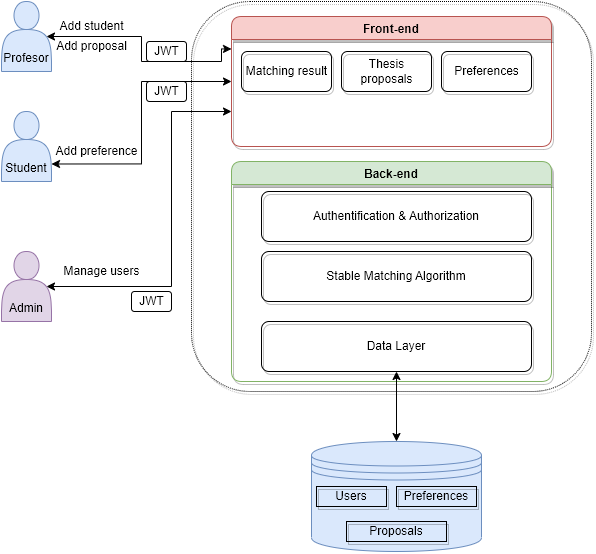
\includegraphics[width=\textwidth, left]{Thesis Matcher-App architecture.drawio.png}
	\caption{Arhitectura aplicației}
\end{figure}
    \chapter{Tehnologii utilizate}

În acest capitol sunt prezentate în primul rând tehnologiile utilizate în implementarea aplicației.

\section{Angular}
\begin{figure}[H]
	
\includegraphics[width=0.3\textwidth, left]{Angular-logo.png}
%	\caption{\url{https://www.vectorlogo.zone/logos/angular/angular-ar21.png}}
\end{figure}

\textbf{Angular} este un framework de JavaScript scris în TypeScript și menținut de Google. Framework-ul a fost dezvoltat în principal pentru crearea aplicațiilor web \textit{single-page}, într-o manieră ce ușurează mentenanța și dezvoltarea ulterioară.

\subsection{Scurt istoric}
În 2010, Miško Hevery, un angajat la Google la acel timp, a lansat un proiect cu numele \textit{AngularJS} care a fost apreciat în mare măsură de comunitate. Între anii 2014-2015 a avut loc o reîmprospăatare majoră a framework-ului însemnând de fapt o rescriere majoră a acestuia. Noua versiune avea să fie numită simplu Angular. Au urmat câțiva ani de tranziție deoarece multe proiecte deja în producție erau utilizau AngularJS și  trebuiau refactorizate. În acest moment, Angular este cel mai folosit framework de front-end, în specialde dezvoltatorii de la Google și de către start-up-uri. Exemple de companii recunoscute ce folosesc Angular sunt Microsoft, Gmail, PayPal, Forbes \cite{angular-history}.

\begin{figure}[H]
	\centering
	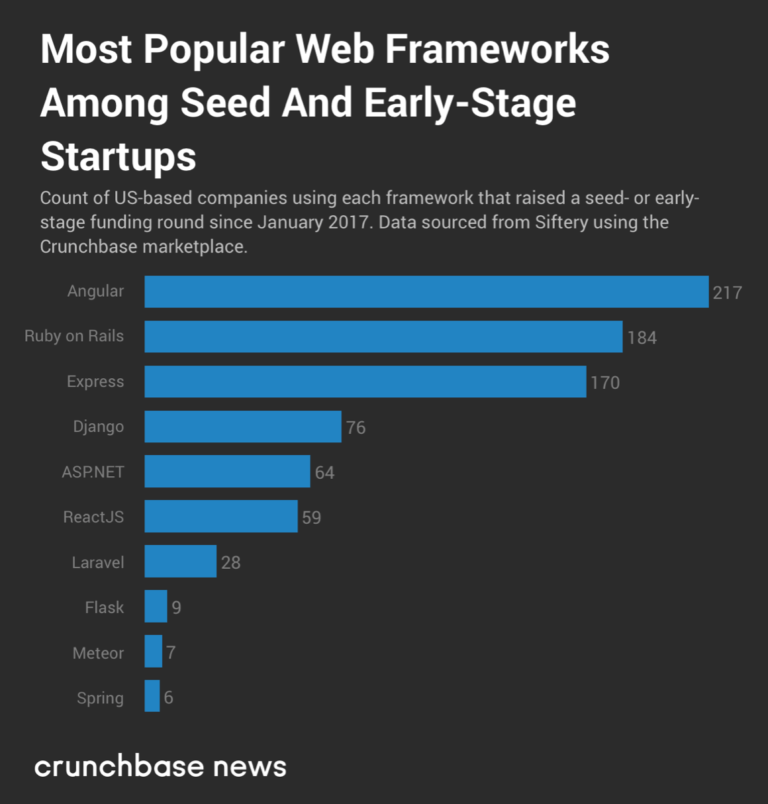
\includegraphics[width=0.8\textwidth]{Angular-crunchbase-newspng.png}
	\caption{\cite{angular-stats}}
\end{figure}

\subsection{Particularități}
Motivul alegerii Angular pe partea de front-end este reprezentat de o serie de caracteristici.

Un astfel de motiv este \textit{arhitectura bazată pe componenta}, fiind astfel o formă de programare orientată pe obiect. Utilizatorul crează în mod uzual clase corespunzătoare componentelor ce conțin și un șablon HTML (\textit{eng.} HTML template). Pentru simplificare, Angular oferă și opțiunea de "injectare" a serviciilor \textit{custom} sau \textit{in-built} într-o componentă ce utilizează aceste funcționalități. În acest fel, utilizatorul poate reutiliza, înlocui, modifica componente în diverse locuri, obținâându-se astfel un UI (User Interface) modularizat.

Un alt motiv este modul de încărcare a paginii web. Angular folosește \textit{lazy loading} ce permite încărcarea instantanee a website-urilor, prin afișarea doar a componentelor cerute și necesare utilizatorului, în timp ce celelalte sunt pregătite în fundal pentru alte eventualități.

\textit{Dependency injection} reprezintă un al treilea motiv, un design pattern ce permite împărțirea lucrului între diferite servicii, distribuind în mod eficient sarcinile. Prin inițializarea dependențelor, Angular reușește să reducă în mod considerabil codul de tip \textit{boilerplate} (fragmente similare de cod des utilizat între care există mici diferențe) și să extindă mai ușor o astfel de aplicație.

Framework-ul are trei tipuri de \textit{dependency injections}:
\begin{enumerate}
	\item Constructor injection
	\item Setter injection
	\item Interface injection
\end{enumerate}

Din punct de vedere al arhitecturii, Angular este în totalitate un framework MVC (model-view-controller), după cum se observă în figura următoare.

\begin{figure}[H]
	\centering
	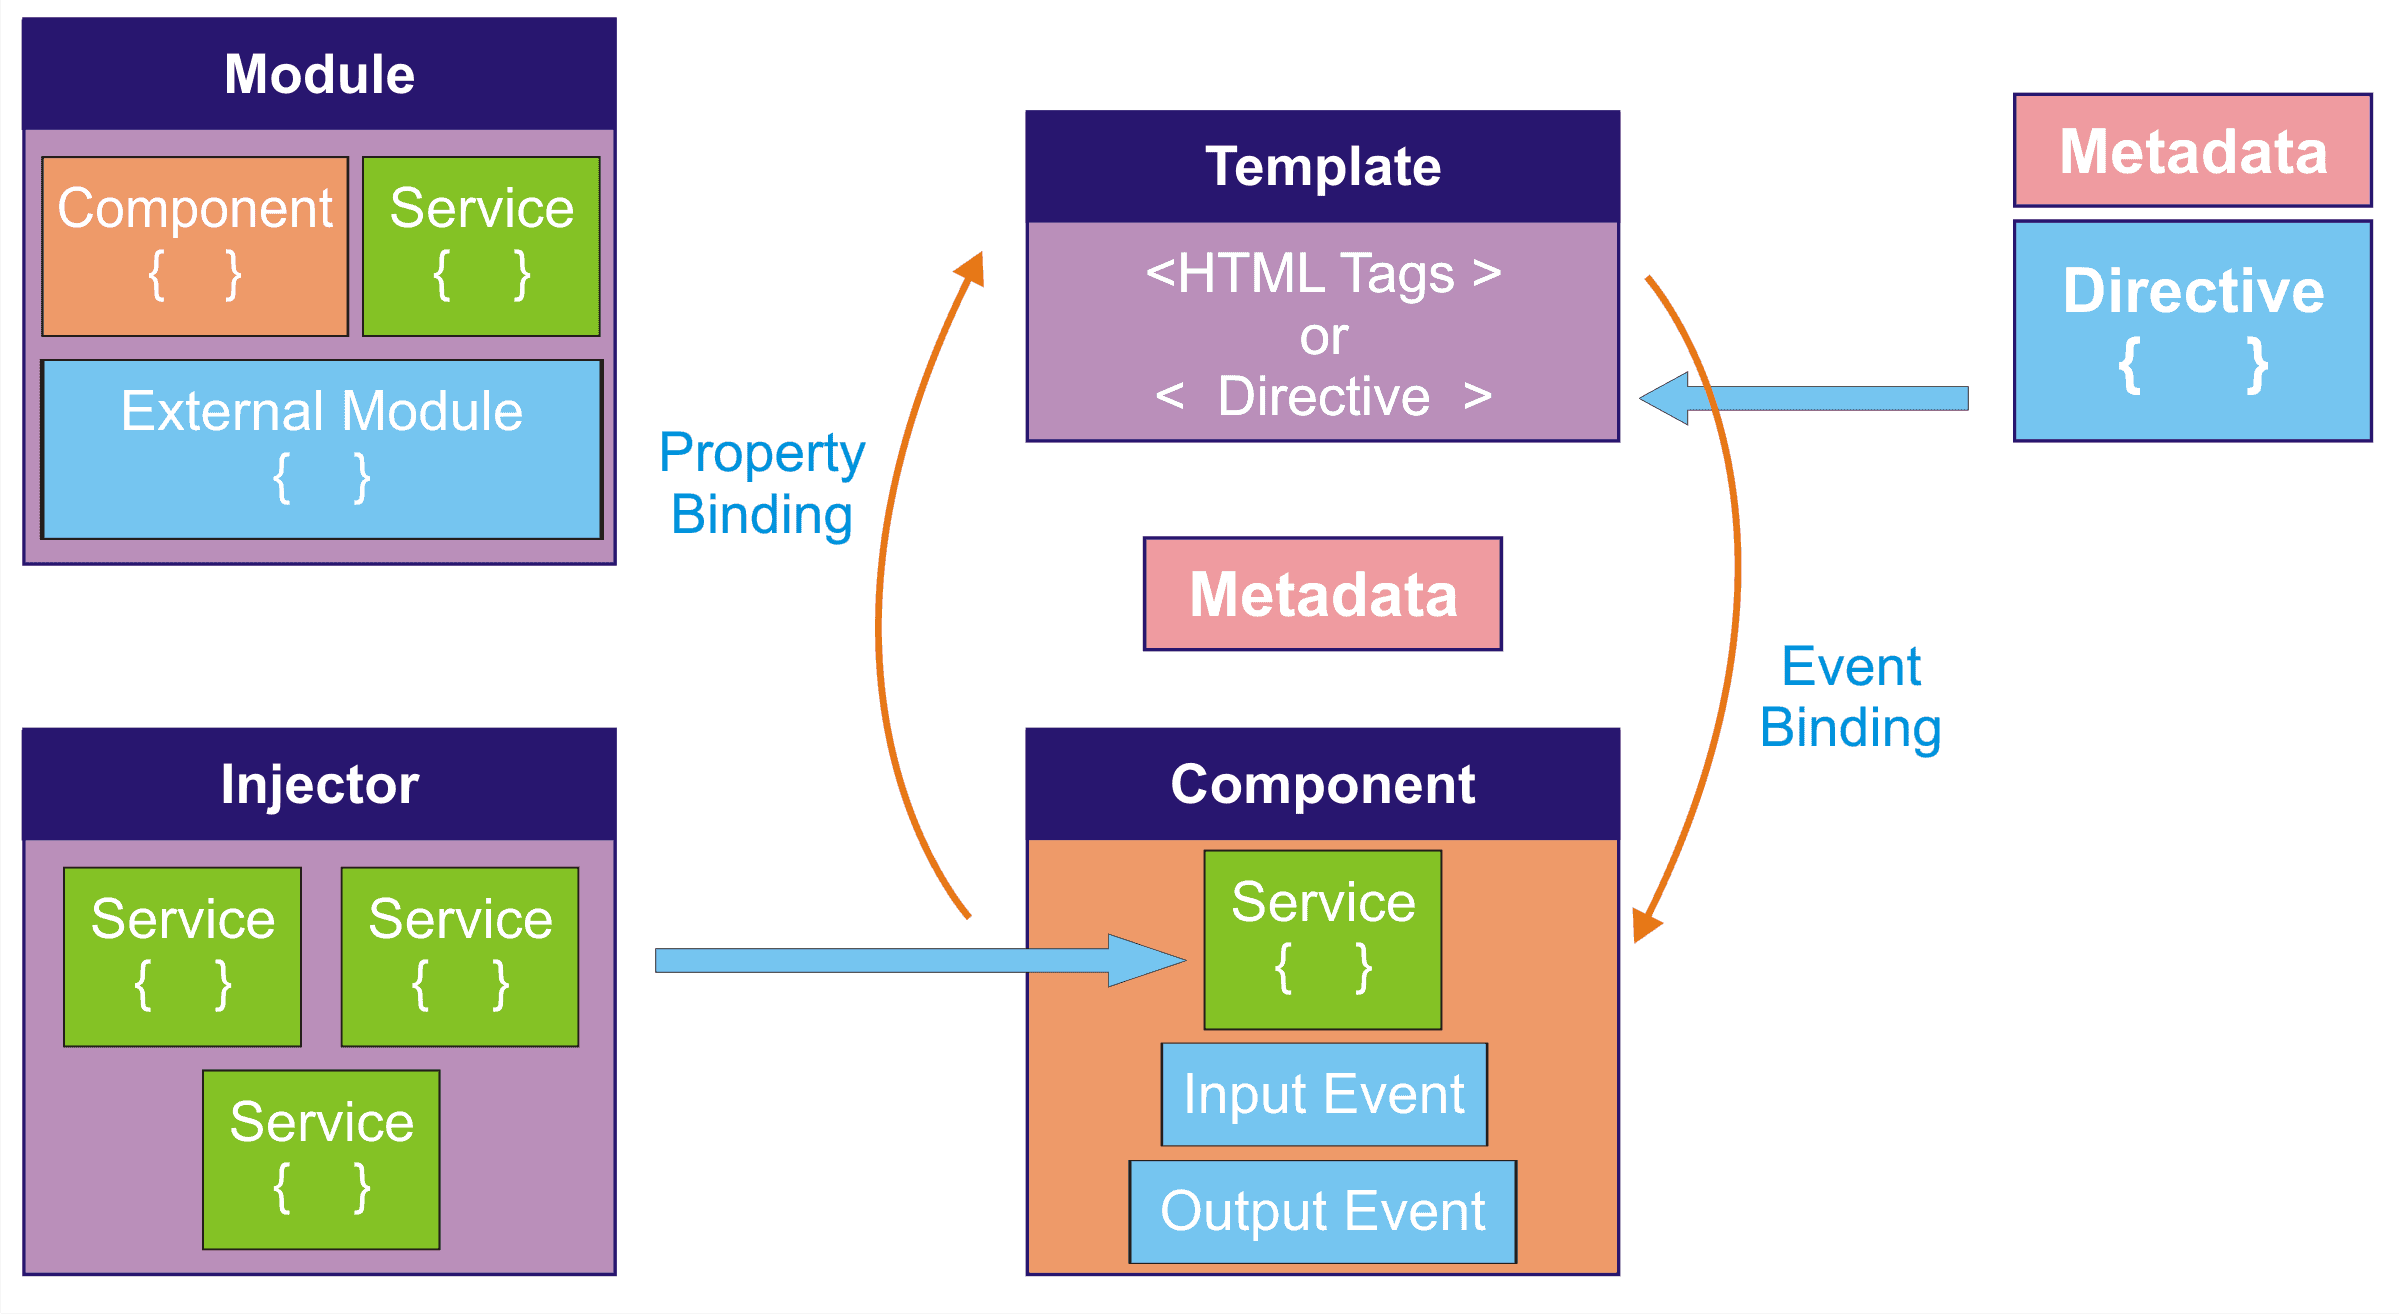
\includegraphics[width=0.8\textwidth]{Angular_Architecture.png}
	\caption{\url{https://www.ngdevelop.tech/wp-content/uploads/2017/12/Angular_Architecture.png}}
\end{figure}

\section{Spring Boot}
\begin{figure}[H]
	\centering
	
\includegraphics[width=0.3\textwidth, left]{Spring-boot-logo.jpg}
%	\caption{\url{https://dev.to/maddy/spring-boot-architecture-547i}}
\end{figure}

\textbf{Spring Boot} este un micro-framework open-source folosit pentru a crea aplicații Spring cu microservicii. Spre deosebire de alte framework-uri de Java, acesta oferă configurări XML flexibile, 
procesare în loturi puternică, tranzacții cu baza de date și o varietate de instrumente de dezvoltare.

\subsection{Scurt istoric}
Framework-ul \textit{Spring} a fost creat în 2004 pentru a simplifica dezvoltarea programelor pe partea de server. În aprilie 2014 a fost lansat Spring boot 1.0.0 în urma unor cereri din partea programatarilor de a configura serviciile de web container într-un container spring din metoda principală. În decembrie 2016 a fost lansat Spring Boot 1.3 ulterior trecerii framework-ului Spring de la versiunea 4.1 la 4.2 și includea sprinjin pentru fisiere JAR complet executabile, noi utilitare spring-boot-dev și auto-configurare pentru tehnologii de caching. 

\subsection{Motivație}
Spring Boot este bazat pe Java, unul dintre cele mai populare limbaje de programare. Framework-ul are o comunitate vastă de utilizatori cu diverse materiale și cursuri.

\begin{figure}[H]
	\centering
	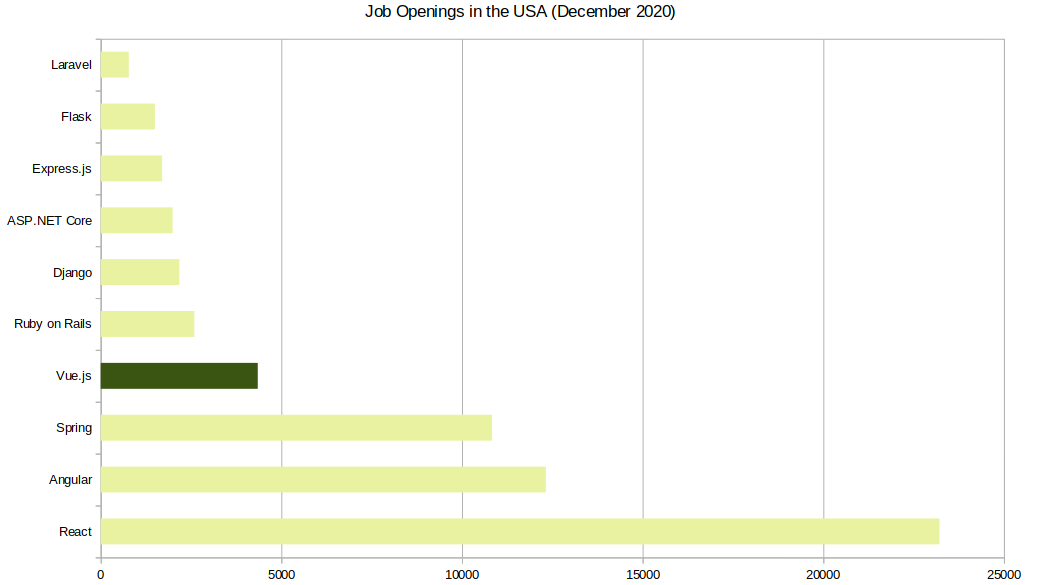
\includegraphics[width=0.8\textwidth]{Spring-ranking.png}
	\caption{\url{https://miro.medium.com/max/1400/1*Y6A_rS5IdRDUG4KRIFP_fA.png}}
\end{figure}

Avantajele prinicipale sunt după cum urmează. Spring Boot este \textit{multi-threaded}, util pentru operații repetitive și de durată. Facilitează crearea și testarea aplicațiilor Java oferind un setup default pentru unit și integration testing. Există de asemenea posibilitatea de a integra Spring Boot cu ecosistemul Spring ce include Spring Data, Spring Security, Spring ORM și Spring JDBC într-un mod simplificat.

\subsection{Particularități}
Principala particularitate a Spring Boot o reprezintă adnotările (\textit{Spring Boot annotations}) utilizate în auto configurare.
De exemplu, \textbf{@SpringBootApplication} marchează metoda principală a aplicației și este obligatorie.
\textbf{@EnableAutoConfiguration} oferă oricărei clase pe care o marchează cu opțiunea de Automatic Configuration.
\textbf{@ComponentScan} scanează la inițializare toate declarările de \textit{beans} și pachete.

Un alt detaliu este utilizarea \textit{Spring Starter Dependencies} ce facilitează gestionarea dependențelor unei aplicații în continuă dezvoltare.

\textit{Spring Boot Actuator} oferă utilitare de producție aplicației. Actuator este utilizat în mare parte pentru a obține informații de funcționare despre o aplicație în rulare (metrice, info, dump, env, etc.), cu ajutorul HTTp endpoints și JMX beans.
Ultima versiune, Spring Boot 2.x Actuator, suportă și modele CRUD.

\subsection{Detalii}
Versiunea de Java este 11.

Versiunea de Spring Boot este 2.7.6.

\section{MySQL}
\subsection{Baza de date}

!!!!!!!!!!!!!!!!!!!!!!!!!!!!!!!!!!!!!!!!!!!!!!!!!!!!!!!!!!!!!!!!!!!!!!!!!!!!!!!!!!!!!!!!!!!!!!!!!!!!!!!!!!!!!!!!!!!!

!!!!!!!!!!!!!!!!!!!!!!!!!!!!!!!!!!!!!!!!!!!!!!!!!!!!!!

\section{Resurse externe}
Datele necesare dezvoltării și testării aplicației printre care se numără studenții, profesorii, preferințele, propunerile (tematici generale sau proiecte particularizate) au fost generate cu ajutorul API-ului \textit{Mockaroo}.
    \chapter{Baza de date}

În acest capitol este argumentată alegerea unui tip de baze de date SQL, mai exact MySQL, pentru a reține informații importante aplicației. A fost preferată o abordare clasică asupra unei baze de date relaționale în special datorită numărului mare de tranzacții ce necesită o asigurare mai mare a integrității datelor \cite{sql1}.

Aplicația \thesistitle este de tip utilitar, aceasta are scopul de a fi folosită într-un context restrâns, în cadrul facultății. Prin urmare numărul de utilizatori este unul relativ mic, reprezentat de către studenți și profesori. De asemenea, poate fi observată o relație strânsă între profesori și propunerile acestora, dar și între studenți și preferințele acestora.

Relațiile între entități sunt de mai multe tipuri, în special \textit{One-to-one} și \textit{One-to-many}. Acest lucru se poate observa în diagrama următoare a bazei de date utilizate.

\begin{figure}[H]
	\centering
	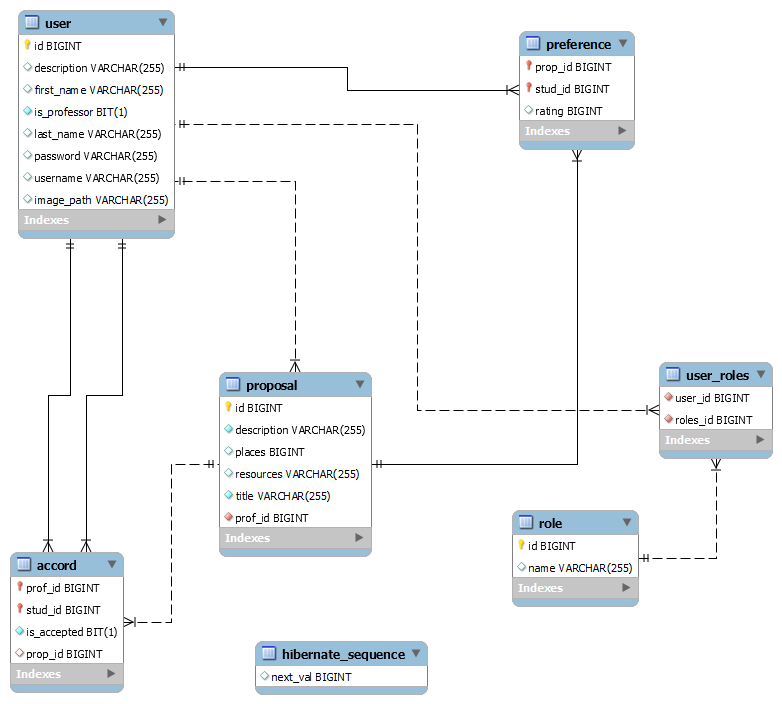
\includegraphics[width=\textwidth, left]{DB_diagram.png}
	\caption{Baza de date}
\end{figure}

În următoarele subcapitole sunt detaliate modelele utilizate pentru a reprezenta aceste date.

\section{Modelarea utilizatorilor}

Utilizatorii au fost modelați într-un mod clasic. Aceștia au la rândul lor roluri în funcție de drepturile pe care le au ei în cadrul aplicației. Astfel, sunt identificate două astfel de roluri: \textbf{ROLE\_USER} și \textbf{ROLE\_ADMIN}. Pe lângă acest lucru, utilizatorii sunt ori profesori, ori studenți, particularitate ilustrată de câmpul boolean \textit{is\_professor} al entității \textbf{\texttt{user}}.

\begin{figure}[H]
	\centering
	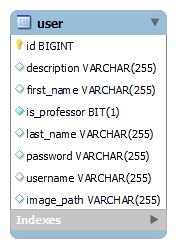
\includegraphics[width=0.3\textwidth, center]{user_model.png}
	\caption{User}
\end{figure}

Fiecare utilizator este identificat unic printr-un \texttt{id} de tipul de date BIGINT, care este și cheie primară a entității. Ca în majoritatea cazurilor, aceștia au un nume de familie (\texttt{last\_name}) și un prenume (\texttt{first\_name}). Câmpul \texttt{username} este de tipul VARCHAR(255) și este reprezentat de un email valid, lucru asigurată pe partea de front-end. Câmpul \texttt{password} este tot de tipul VARCHAR(255) și reprezintă parola utilizatorului, însă criptată pe partea de back-end cu un algoritm clasic.
Aceste două câmpuri sunt primite de către utilizator din partea unui administrator și sunt utilizate pentru autentificarea în aplicație. A fost preferată această abordare pentru a împiedica crearea de conturi din partea unor persoane din afara contextului.

\subsection{ROLE\_USER}

Cei mai mulți utilizatori au rolul \textbf{ROLE\_USER}, un rol default. Acest lucru le autorizează accesul la aplicație, odată ce aceștia sunt autentificați. Interfața diferă în funcție de tipul utilizatorului.

\subsubsection{Tipuri}

\textbf{Profesorii} pot crea și actualiza propuneri (en. proposals) pentru teza de licență. Aceste propuneri pot fi \textit{project} sau \textit{topic}, detalierea acestora urmând a fi făcută ulterior. De asemenea, aceștia pot încheia acorduri (en. accords) cu anumiți studenți pentru unele dintre propunerile lor. Acest lucru le permite studenților să nu mai participe la algoritmul de stable matching, fiind deja repartizați profesorilor respectivi.

\textbf{Studenții} pot crea și actualiza preferințe (en. preferences) într-o anumită ierarhie a lor. Așadar, categorisirea utilizatorilor în profesori și studenți are unicul scop de a diferenția interfața în funcție de funcționalitățile specifice tipurilor acestora.


\subsection{ROLE\_ADMIN}

Există în plus un număr restrâns de utilizatori care au rolul de administrator, \textbf{ROLE\_ADMIN}. Aceștia au dreptul de a gestiona conturile participanților, mai precis de a crea, actualiza și elimina utilizatorilor. De asemenea, administratorii au opțiunea de a impune anumite limite în cadrul aplicației cum ar fi o limită a propunerilor pentru profesori și o limită a preferințelor pentru elevi.

\section{Preferințele}

Preferințele sunt modelate simplu, reprezentând în sine o relație între entitățile studenți și propuneri.

\begin{figure}[H]
	\centering
	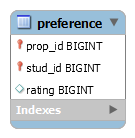
\includegraphics[width=0.3\textwidth, center]{preference_model.png}
	\caption{Preference}
\end{figure}

După cum se poate observa în tabela \textbf{\texttt{preference}}, acestea cuprind un \texttt{id\_stud} ce face legătura cu tabela \textbf{\texttt{student}} și un \texttt{id\_prop} ce face legătura cu tabela \textbf{\texttt{proposals}}.

În plus, există un câmp \texttt{rating} care este de tipul BIGINT și indică invers proporțional importanța preferinței, mai exact o preferință cu un $\texttt{level} = 0 $ este pe primul loc în ierarhie. Este de asemenea important de precizat că mai multe preferințe ale unui student pot avea același rating, lucru necesar pentru un algoritm de \textit{stable matching with ties}.

Aceste relații între studenți și tezele propuse vor constitui datele de intrare pentru algoritm, fiind astfel de o importanță semnificativă în cadrul aplicației.

\section{Propunerile}

În cazul propunerilor, la nivel teoretic acestea pot fi de două tipuri, proiect (en. project) sau temă (en. topic). Diferența constă în faptul că un proiect este o propunere mai concisă, cu o descriere exactă a lucrării așteptate, fie ea una de cercetare sau o aplicație propriu-zisă, iar un proiect nu poate fi ales și realizat decât de către o singură persoană.
Un astfel de exemplu ar putea fi \textit{„Realizare unei aplicații de reconoaștere facială utilizând metode de machine learning”}, cu precizările și restricțiile aferente.

Pe de altă parte, o temă este o descriere pe larg a anumitor particularități ale unui proiect de cele mai multe ori dintr-un anumit domeniu de specialitate. La fel ca un proiect specific, o temă poate cuprinde atât lucrări general teoretice, cât și practice, studentul fiind nevoit să stabilească împreună cu profesorul său coordonator o teză concretă. Însă o propunere de acest fel poate avea un număr de locuri disponibile mai mare de 1, deoarece mai mulți studenți pot urma direcții diferite asupra tematicii propuse. Spre exemplu, profesorul poate propune o temă de „Algoritmi genetici și optimizarea acestora” care poate fi repartizată unor 3 studenți care stabilesc în mod distinct cu profesorul de licență lucrările lor.

Cu toate acestea, din motive de simplificare și optimizare, la nivelul de scehmei de baze de date, a preferată modelarea propunerilor într-o singură tabelă intitulată sugestiv \textbf{\texttt{proposal}}, diferența dintre cele două tipuri fiind făcută de câmpul \texttt{places}. 

\begin{figure}[H]
	\centering
	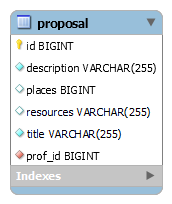
\includegraphics[width=0.3\textwidth, center]{proposal_model.png}
	\caption{Proposal}
\end{figure}

În cazul proiectelor (projects) câmpul acesta rămâne \texttt{null}, spre deosebire de teme (topics). Fiecare propunere are un titlu (\texttt{title}) reprezentativ și o descriere (\texttt{description}) adecvată de tipul VARCHAR(255), precum și o listă de referințe pentru a ajuta studentul. Ultimul câmp este \texttt{id\_prof} care indică autorul propunerii.


\section{Acordurile}

În cadrul aplicației \thesistitle, fiecare profesor poate stabili împreună cu un student un acord, reprezentat de tabela cu același nume \textbf{\texttt{accord}}, în ideea că acest student și propunerea aleasă nu mai sunt luate în calcul la rularea algoritmului de repartizare. Cu alte cuvinte, acest detaliu le permite studenților posibilitatea să realizeze un proiect preferat, adecvat abilităților și înclinațiilor sale, desigur cu aprobarea profesorului corespunzător tezei alese.

\begin{figure}[H]
	\centering
	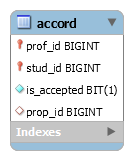
\includegraphics[width=0.3\textwidth, center]{accord_model.png}
	\caption{Accord}
\end{figure}

\section{Lucrul pe partea de back-end cu baza de date}

Partea de back-end a aplicației, fiind implementată cu ajutorul Spring Boot, interacționează cu baza de date prin intermediu Hibernate, alegere făcută luând în considerare o serie de avantaje.

\subsection{Hibernate}

\begin{figure}[H]
	
\includegraphics[width=0.3\textwidth, left]{hibernate-logo.png}
	\caption{\url{https://hibernate.org/images/hibernate-logo.svg}}
\end{figure}

\subsubsection{Ce este Hibernate}

Hibernate este un framework, mai precis un ORM (object relational mapping) creat pentru a facilita maparea modelelor orientate-obiect la baze de date relaționale pentru aplicații web \cite{hibernate1}. În mod intern, acest ORM utilizează JDBC API pentru a interacționa cu baza de date \cite{hibernate2}.

\begin{figure}[H]
	\centering
	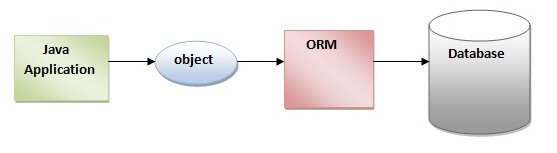
\includegraphics[width=0.3\textwidth, center]{orm.jpg}
	\caption{ORM}
\end{figure}

Hibernate este cu alte cuvinte o implementare a specificațiilor JPA (Java Persistence API) pentru persistența datelor. JPA este un set de reguli care oferă un standard definit și o anumită funcționalitate acestor tehnologii ORM \cite{hibernate2}.

\subsubsection{Funcționalitatea Hibernate}

Framework-ul precizat corelează clase din limbajul Java tabelelor din serverul de baze de date, dar și tipurile de date din Java cu cele din SQL pentru a asigura persistența obiectelor. Hibernate returnează astfel aplicației enitățile sub formă de obiecte Java și reduce astfel timpul de procesare a rezultatelor și codul necesar implementat de programator.

\subsubsection{Avantaje ale Hibernate}

Hibernate este în primul rând un framework \textit{open source} și \textit{lightweight}, lucru ce mi-a permis familiarizare cu acesta și ușoara configurare a lui.

În al doilea rând, Hibernate este un framework relativ rapid deoarece beneficiază de un cache intern, structurat pe două niveluri, primul nivel fiind folosit în mod normal \cite{hibernate2}.

De asemenea, tehnologia optată utilizează o versiune orientată obiect a SQL-ului, HQL (Hibernate Query Language), care permite generează query-uri independente de baza de date, fără a scrie în mod explicit query-uri în SQL \cite{hibernate2}.

În final, Hibernate oferă posibilitatea de a crea și popula tabelele din baza de date în mod automat, direct din cod.

Imaginea următoare ilustrează specificațiile din fișierul \texttt{application.properties} specific oricărui proiect Maven, în care sunt este configurată utilizarea framework-ului Hibernate. Acest lucru include date de conectare la baza de date, modul de conectare, dialectul SQL folosit etc.

\begin{figure}[H]
	\centering
	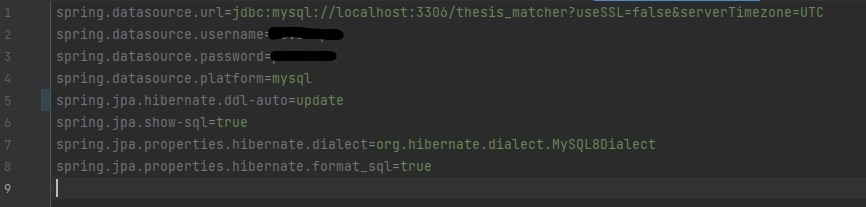
\includegraphics[width=\textwidth, left]{application-properties.jpg}
	\caption{application.properties}
\end{figure}

Pentru a putea folosi Hibernate într-un proiect de Spring Boot este necesară adăugarea dependenței următoare în fișierul \texttt{pom.xml}.

\begin{figure}[H]
	\centering
	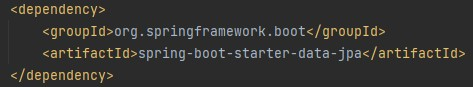
\includegraphics[width=\textwidth, left]{hibernate-dependency.jpg}
	\caption{Dependența din pom.xml}
\end{figure}

\section{Generarea datelor}

În vederea generării unor date reprezentative problemei actuale, a fost creată o clasă separată numită \texttt{Populator} ce introduce înregistrări (records) în baza de date. De aceea au fost stabilite în primul rând o serie de parametri care reglează dimensiunile populațiilor și proporțiile dintre diferitele tipuri de entități. În continuare vor fi prezentați pe scurt acești parametri și configurarea lor, urmând a descrie maniera de generare propriu-zisă a utilizatorilor, propunerilor profesorilor și nu în ultimul rând, preferințelor studenților.

Configurarea parametrilor necesari generării datelor este realizată prin intermediul unei clase \texttt{PopulatingConfiguration}.

\begin{figure}[H]
	\centering
	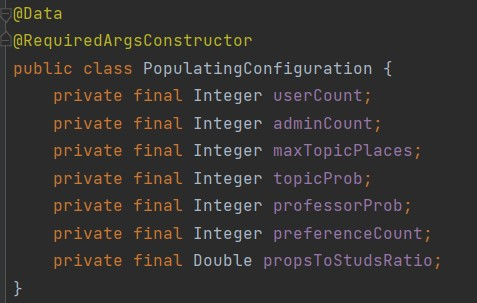
\includegraphics[width=0.6\textwidth, left]{populating-config-class.jpg}
	\caption{Clasa de parametri de configurare}
\end{figure}

Aceasta conține parametri precum numărul de utilizatori (\texttt{userCount}), numărul de administratori (\texttt{adminCount}), probabilitatea ca un utilizator să fie profesor 
(\texttt{professorProb}) etc.

Primul pas este generarea utilizatorilor. Pentru această etapă a fost folosită clasa \texttt{Faker} în obținerea unor nume aleatorii. Parola tuturor a fost setată aceeași pentru simplificare, iar primi \texttt{adminCount} utilizatori primesc \texttt{ROLE\_ADMIN} pe lângă \texttt{ROLE\_USER}.

Cel de al doilea pas este generarea propunerilor pentru fiecare profesor ales dintre utilizatori conform unei probabilități. Se calculează întâi un număr de locuri în corelație cu numărul de studenți ce trebuie acoperit de fiecare profesor pentru a putea da șansa unei repartizări a tuturor studenților. De menționat că tipul propunerilor este tot ales aleatoriu.

Ultimul pas este crearea preferințelor și a acordurilor utilizatorilor.
    \chapter{Front-end}

Pentru partea de front-end a aplicației a fost ales framework-ul de Typescript Angular datorită unor mai multe avantaje. O particularitate importantă și principală a acestui framework este faptul că utilizează componente pentru crearea unei aplicații \textit{single-page}.

Astfel, posibilitatea de creare a componentelor permite reutilizarea acestora și economisirea codului, aplicația devenind una orientată-obiect datorită și faptului că aceste componente sunt implementate în Typescript, un limbaj \textit{strongly typed} dezvoltat din Javascript.

Nu în ultimul rând, familiarizarea cu această tehnologie are loc relativ repede, iar documentația vastă alături de diversele cursuri și tutoriale permit o învățare adecvată și dezvoltarea unor soluții optime.

\section{Interfața}

Interfața este adaptată în funcție de tipul de utilizator autentificat. Există elemente comune în general, dar și anumite funcționalități specifice.

\subsection{Pagina principală}

Prima pagină a aplicației \thesistitle{} este cea de \textbf{Matching}, vizibilă oricărui utilizator, indiferent de tipul său sau dacă este autentificat sau nu.

\begin{figure}[H]
	\centering
	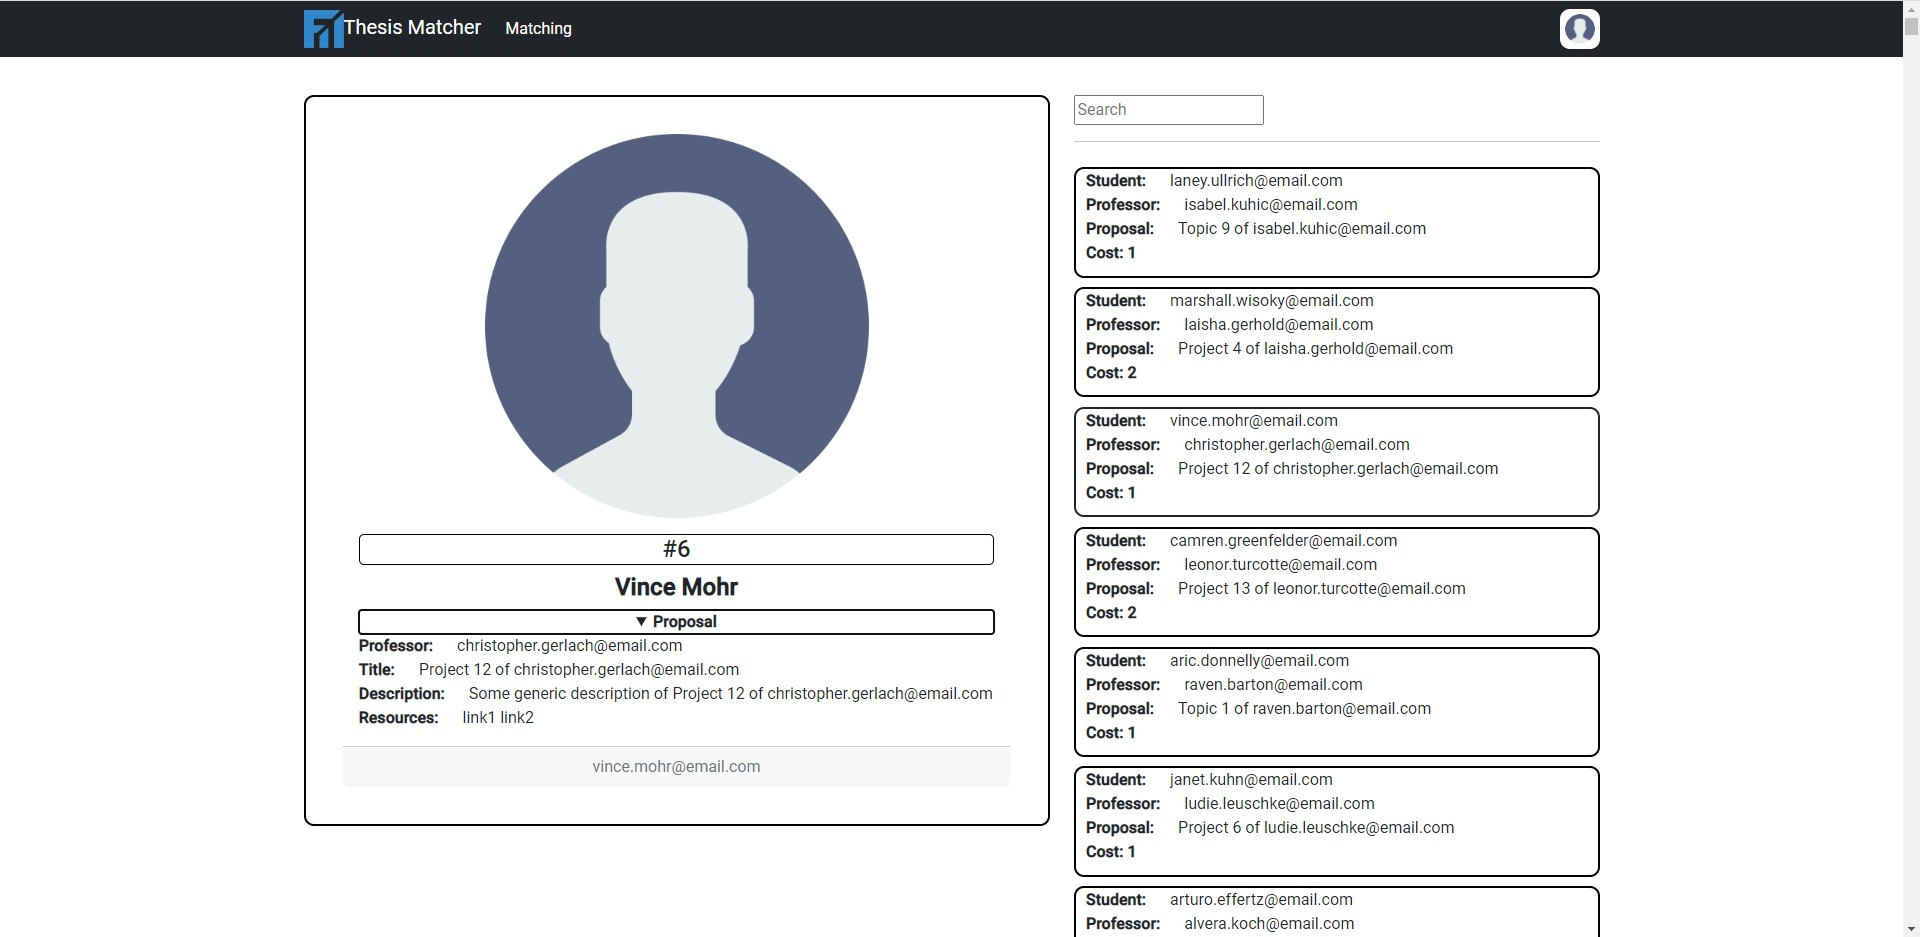
\includegraphics[width=1\textwidth, center]{matching-page.jpg}
	\caption{Matching (repartiția)}
\end{figure}

Aici se poate observa lista tuturor studenților și propunerea (proiectul sau tematica) asignată fiecăruia în funcție de preferințele sale. De asemenea, pentru fiecare asignare este înregistrat un \textit{cost} care indică locul propunerii primite în ordinea preferințelor sale (de exemplu, o asignare cu costul 1 înseamnă că propunerea a fost pe primul loc în lista sa, o alta cu costul 2 a fost pe al doilea loc etc.). În plus, există o opțiune de a căuta prin rezultat după numele studentului, al profesorului sau titlul lucrării.

Totuși, opțiunile utilizatorului sunt mult restrânse, lucru ce se poate observa și din bara de navigare, el fiind nevoit să se autentifice.

Pagina de autentificare este simplă, utilizatorul fiind nevoit să introducă email-ul și parola unui cont existent după cum se poate obeserva în figura următoare.

\begin{figure}[H]
	\centering
	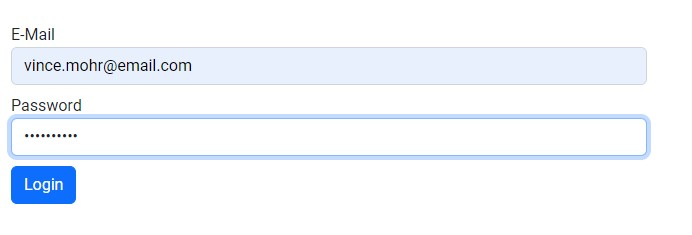
\includegraphics[width=0.5\textwidth, center]{auth-page.jpg}
	\caption{Pagina de autentificare}
\end{figure}

Odată autentificat, utilizatorul își poate schimba fotografia de profil, descrierea în care poate specifica domeniile de interes. În plus, acesta își poate schimba parola de la cont. Toate aceste setări pot fi efectuate din pagina \textbf{My Profile}.

\begin{figure}[H]
	\centering
	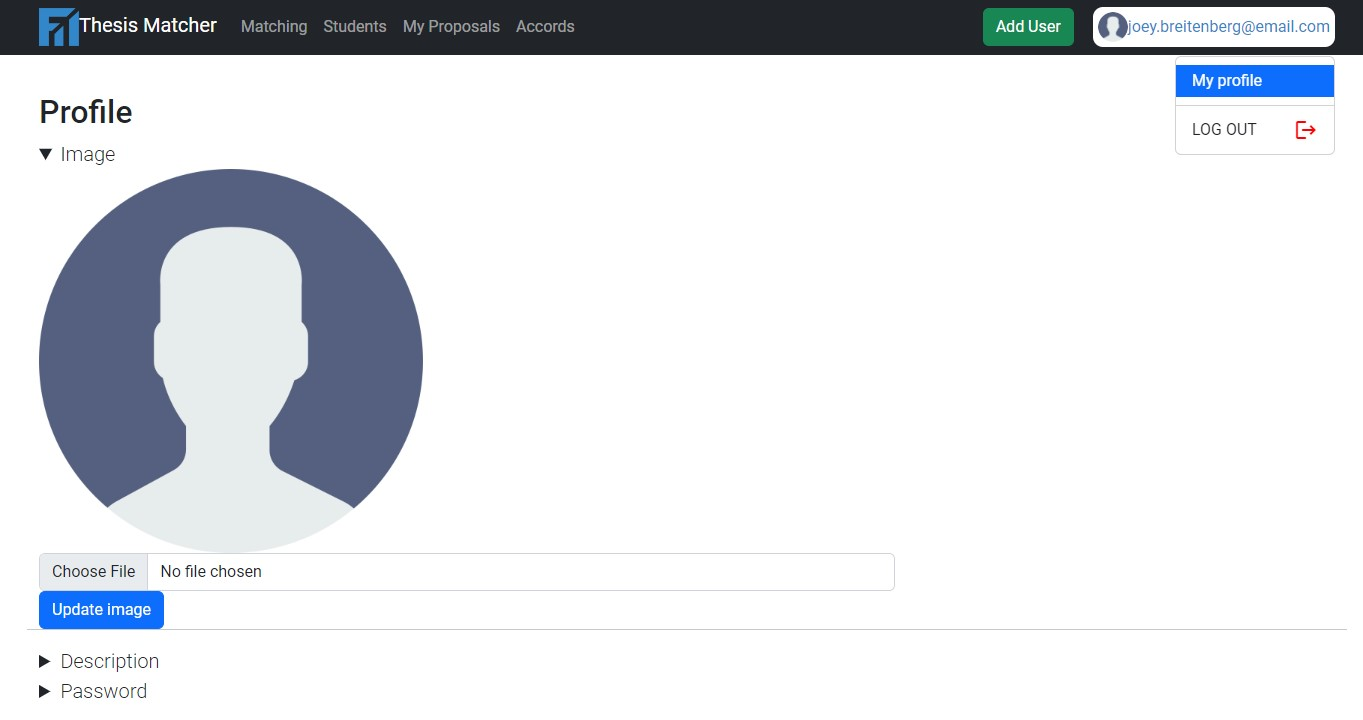
\includegraphics[width=0.5\textwidth, center]{my-profile-page.jpg}
	\caption{Profilul utilizatorului}
\end{figure}

\subsection{Interfața studentului}

Un utilizator de tip \textit{student} poate accesa pagina \textbf{Professors} unde poate vedea detalii despre fiecare profesor, însă principalul scop al acestei pagini este de a accesa propunerile fiecărui profesor în parte.

\begin{figure}[H]
	\centering
	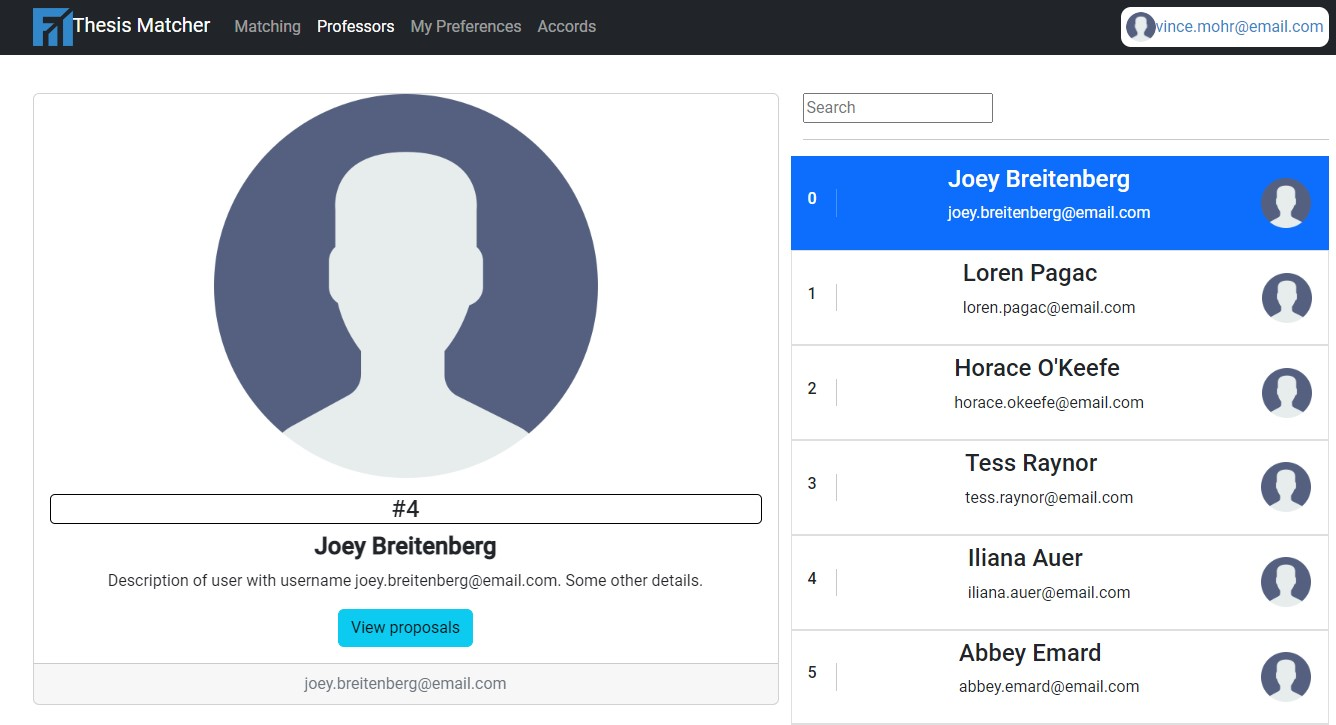
\includegraphics[width=0.5\textwidth, center]{professors-page.jpg}
	\caption{Profesorii}
\end{figure}

\begin{figure}[H]
	\centering
	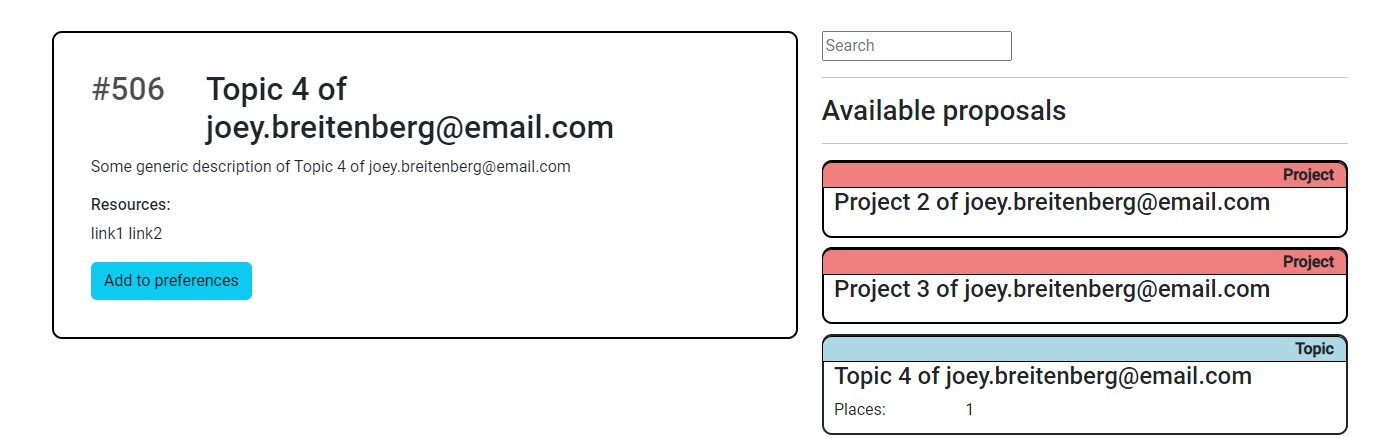
\includegraphics[width=0.5\textwidth, center]{proposals-page.jpg}
	\caption{Propunerile unui profesor}
\end{figure}

Acest lucru permite adăugarea unei propuneri la lista sa de preferințe. El poate căuta în lista de propuneri a profesorului respectiv după titlu sau descriere. Pentru a marca și diferenția opțiunile între ele după tip, proiectele au fost colorate cu roșu, iar tematicile (topics) în albastru, acestea având specificat și un număr limită de locuri disponibile, spre deosebire de proiecte care au câte unul singur. 

Pagina preferințelor (\textbf{Preferences}) conține toate propunerile apreciate de către student. Acesta poate elimina de exemplu un proiect din listă sau poate modifica rating-ul, un număr întreg între 1 și 100. După cum a fost deja menționat, două preferințe pot avea același rating, iar acest număr este utilizat strict pentru ordonarea preferințelor. Atunci când este adăugată o preferință, aceasta are inițializat rating-ul cu 1, fiind la finalul ierarhiei.

\begin{figure}[H]
	\centering
	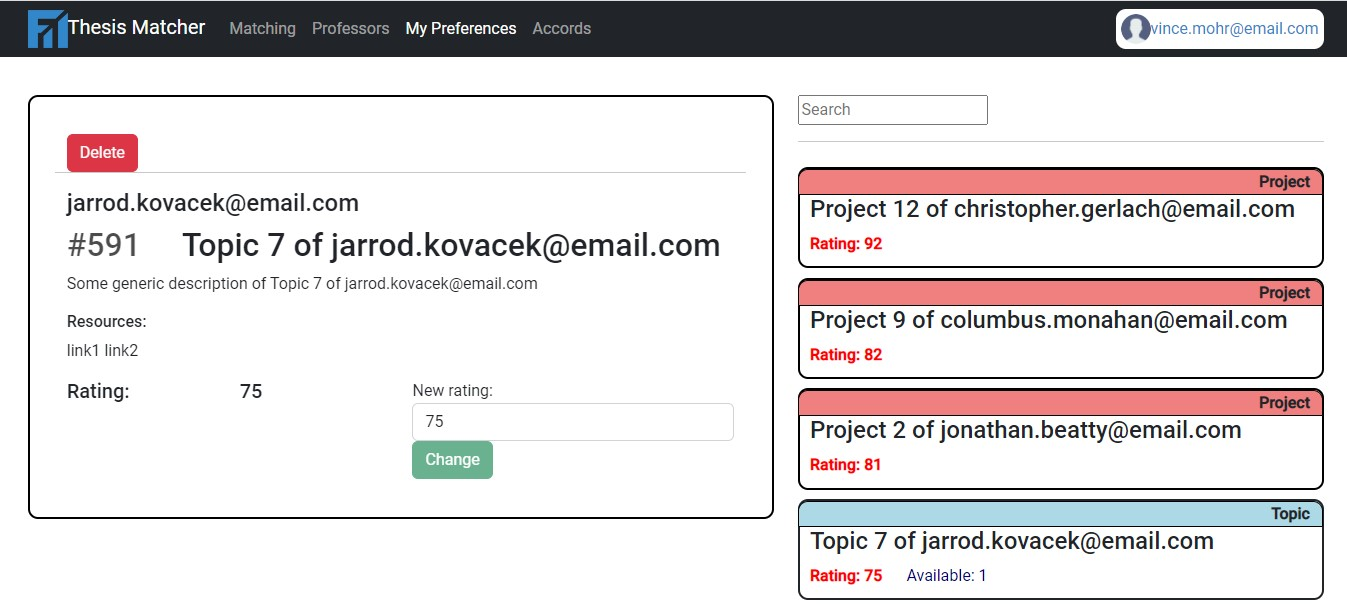
\includegraphics[width=0.6\textwidth, center]{preferences-page.jpg}
	\caption{Preferințele}
\end{figure}

\subsection{Interfața profesorului}

Interfața unui profesor este în mare măsură similară. În pagina \textbf{Students} el poate vedea o listă de studenți și iniția un acord pentru o anumită lucrare, adică să asigneze un proiect sau o tematică unui student.

Pagina \textbf{My proposals} cuprinde propunerile create de profesor. Acesta poate adăuga noi proiecte, modifica elemente deja existente sau să le elimine.

\begin{figure}[H]
	\centering
	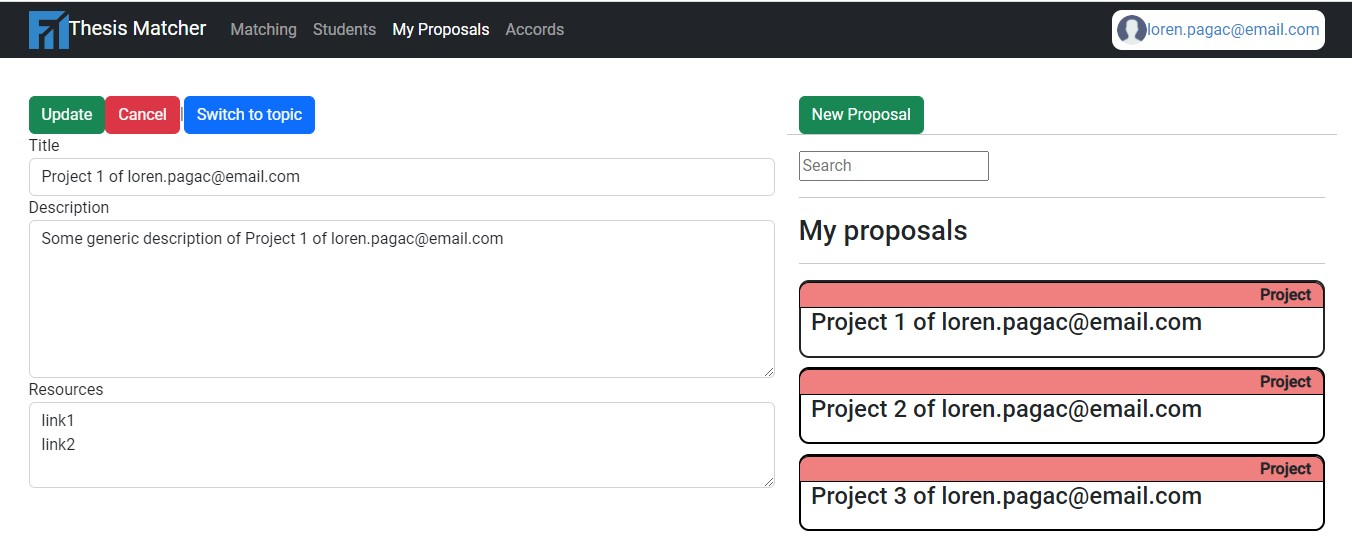
\includegraphics[width=0.6\textwidth, center]{professor-proposals-page.jpg}
	\caption{Propunerile}
\end{figure}

În secțiunea \textbf{Accords} există toate acordurile inițiate de către profesor. Pentru a fi luat în calcul, un acord trebuie însa acceptat de către student. În acest fel, studentului i se asignează deja un proiect, iar în acest fel atât acesta, cât și propunerea, nu mai intră în pasul de determinare a unei repartizări. Acordurile acceptate sunt marcate cu verde, în caz contrar, cu roșu.

\begin{figure}[H]
	\centering
	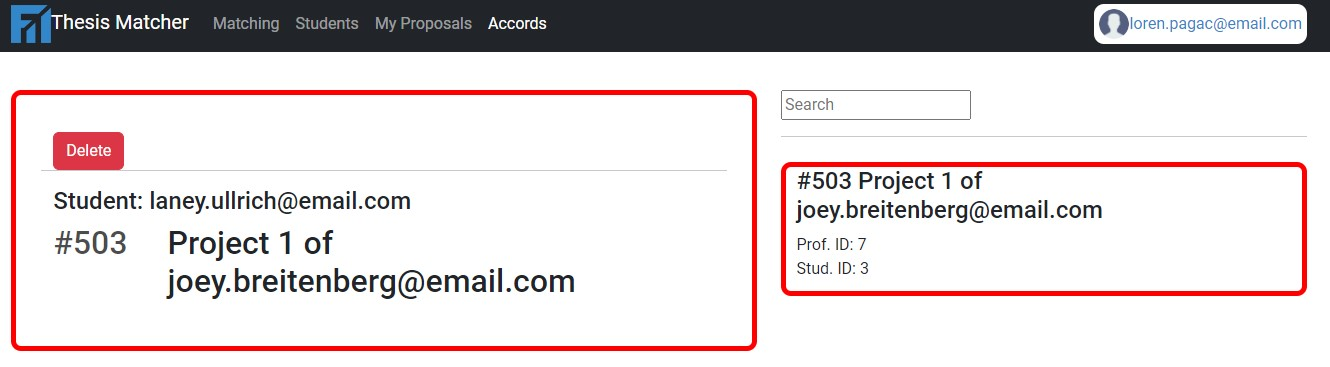
\includegraphics[width=0.6\textwidth, center]{accords-page.jpg}
	\caption{Acordurile}
\end{figure}

\subsection{Administratorul}

În cadrul acestei aplicații, fiind proiectată ca utilitar de uz intern, doar utilizatorii cu drepturi de administrator (ROLE\_ADMIN) pot adăuga noi utilizatori. Prin urmare, doar aceștia au acces la pagina \textbf{Add User} de unde pot realiza acest lucru.

\begin{figure}[H]
	\centering
	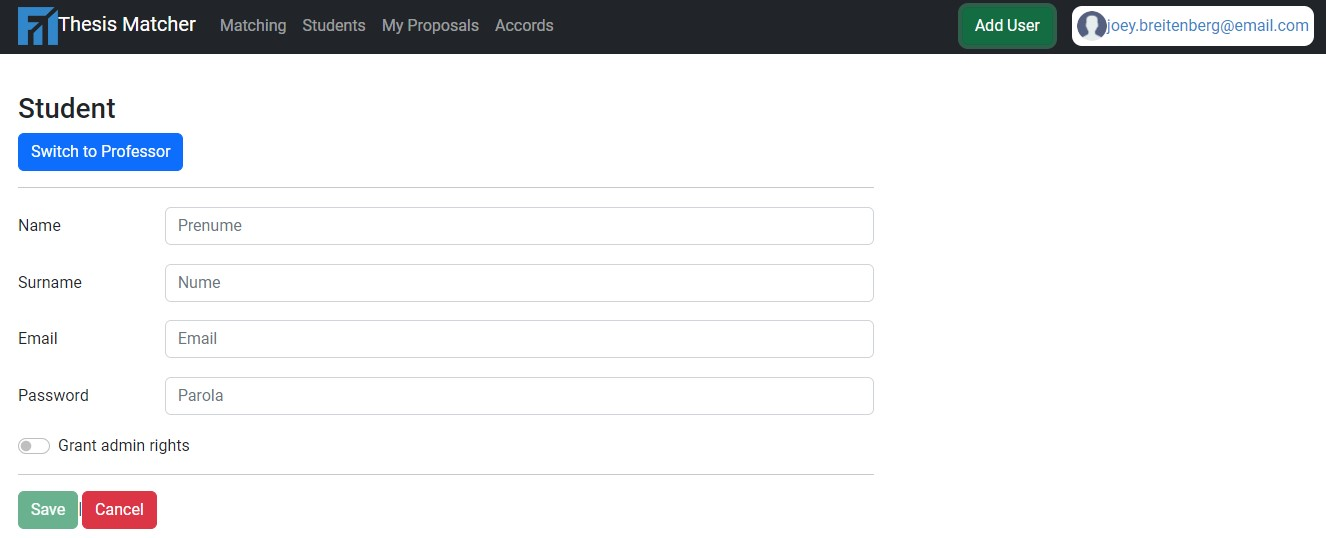
\includegraphics[width=0.6\textwidth, center]{add-user-page.jpg}
	\caption{Adăugarea unui utilizator}
\end{figure}

\section{Detalii de implementare}

Înainte de a prezenta implementarea generală a părții de front-end, este necesară explicarea alcătuirii unei componente Angular.

Componenetele sunt elementele de bază ale interfeței unei aplicații Angular, o astfel de aplicație conține un arbore de componente \cite{component1}. Acestea sunt de fapt din puct de vedere tehnic un tip de directive, întotdeauna asociate cu un template.

O componentă este alcătuită dintr-un fișier Typescript ce modelează componenta prin intermediul unei clase, un \textit{template} (șablon) ce descrie cum este construită (\textit{rendered}) aceasta și eventual un fișiser CSS care indică detalii de stilizare.

\subsection{Lifecylce hooks}

Fiecare componentă are un ciclu de viață (lifecycle) care începe odată cu instanțierea și afișarea acesteia, continuă cu detectarea schimbărilor în view și în proprietățile instanței și se termină cu distrugerea componentei și eliminarea acesteia din DOM \cite{angular-lifecycle}.

Există posibilitatea de a răspunde la astfel de evenimente din ciclul de viață al unei componente prin intermediul unor interfețe precum OnInit sau OnDestroy.

\begin{figure}[H]
	\centering
	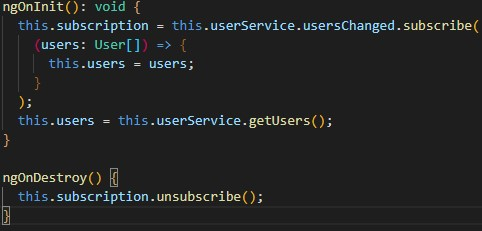
\includegraphics[width=0.6\textwidth, center]{user-list-on-init.jpg}
	\caption{Metodele ngOnInit și ngOnDestroy în componenta UserList}
\end{figure}

Se poate observa cum în metoda \texttt{ngOnInit} a componentei \texttt{UserList} sunt efectuate operații necesare instanțierii și afișării listei de utilizatori. Utilizând serviciul \texttt{userService} injectat în constructor, se crează un obiect de tipul \texttt{Subscription} pentru a obține un tablou de utilizatori. În metoda \texttt{ngOnDestroy}, acest obiect este înlăturat pentru a optimiza folosirea memoriei.

\subsection{Accesarea unei rute}

Angular este utilizat în principal pentru crearea de aplicații \textit{single-page}, adică toate funcționalitățile există într-o singură pagină HTML. Browser-ul încarcă doar părțile (componentele) necesare utilizatorului, fără a încărca o nouă pagină. De aceea, utilizatorul navighează prin intermediul rutelor predeterminate \cite{angular-routes}. Acestea permit afișarea unor view-uri specifice în funcție de calea URL. Pentru a dispune de această funcționalitate, trebuie importat modulul \texttt{RouterModule} din pachetul \texttt{@angular/router}.

Rutele sunt stabilite în acest caz în modulul \texttt{AppRoutingModule}, iar definiția unei rute este din punct de vedere tehnic un obiect JavaScript \cite{angular-routes}. Fiecare are măcar proprietățile \texttt{path} ce indică calea URL și \texttt{component}, numele componentei afișate. Definirea este realizată în manieră ierarhică, fiecare rută putând avea o listă de descendenți. Spre exemplu, în imaginea următoare se poate vedea rutele necesare vizualizării propunerilor, a detaliilor unui anumit element, adăugarea și modificarea unei propuneri.

\begin{figure}[H]
	\centering
	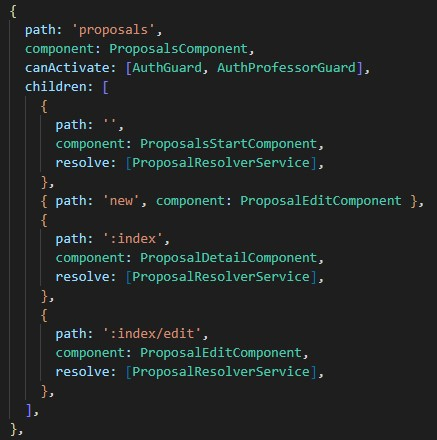
\includegraphics[width=0.5\textwidth, center]{proposals-routes.jpg}
	\caption{Rutele pentru propuneri}
\end{figure}

\subsection{Serviciile}

În cadrul acestei aplicații, serviciile sunt o parte esențială în special în comunicarea dintre componente și transmiterea și primirea de informații către/de la back-end. Fiecare serviciu este adnotat cu \texttt{Injectable} pentru a permite injectarea acestora în alte obiecte.

În figura următoare este prezentată parțial implementarea serviciului de autentificare.

\begin{figure}[H]
	\centering
	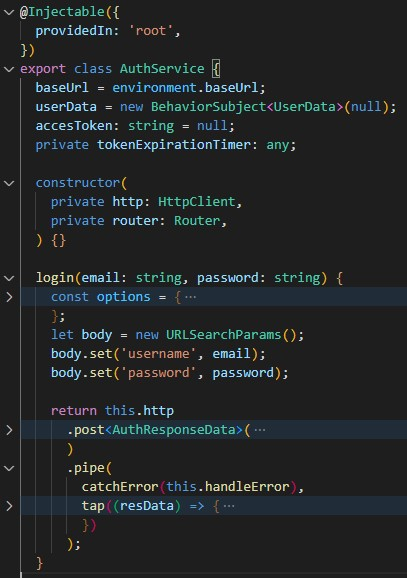
\includegraphics[width=0.4\textwidth, center]{auth-service.jpg}
	\caption{Serviciul de autentificare}
\end{figure}

Acesta utilizează la rândul său serviciile \texttt{HttpClient} pentru comunicarea cu back-end-ul prin request-uri HTML și \texttt{Router} pentru navigare. Astfel, în metoda \texttt{login} este efectuat un request \texttt{POST}, cu \textit{body} de tipul \texttt{x-www-form-urlencoded} (specificat în \textit{headers}) conținând câmpurile \textit{username} și \textit{password} cu valorile aferente. Rezultatul acestui request este un obiect de tipul \textit{AuthResponseData} ce conține în special câmpul \textit{accessToken}. Acest token este un șir de caracter reprezentând un JWT (JSON Web Token) și este unic fiecărui utilizator și necesar pentru efectuarea cu succes a oricărui request ulterior.

Un alt detaliu este reprezentat de variabila \texttt{userData}, de tipul \textit{BehaviourSubject<UserData>}, care permite emiterea unor evenimente pentru a indica autentificarea și dezautentificarea utilizatorului.

\subsubsection{Resolver}

Un categorie particulară a serviciilor este cea de \textbf{Resolvers}. Un astfel de serviciu implementează interfața \textit{Resolve} și este utilizat pentru operații premergătoare încărcării unei componente, iar specificarea acestui are loc în \texttt{AppRoutingModule}. În cazul propunerilor, prin intermediu serviciului \texttt{ProposalService} este obținută o listă completă a propunerilor profesorului autentificat.

\begin{figure}[H]
	\centering
	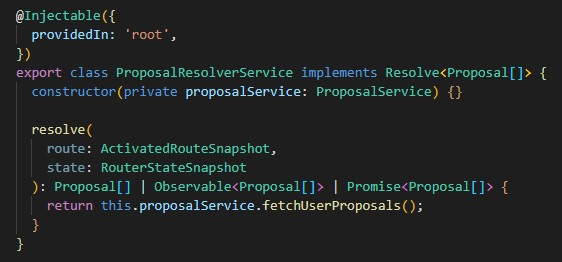
\includegraphics[width=0.5\textwidth, center]{proposal-resolver.jpg}
	\caption{Resolver pentru propuneri}
\end{figure}

\subsubsection{Guard}

O altă categorie este cea a gărzilor sau \textbf{Guards} în engleză, care autorizează accesul utilizatorilor la diversele rute în conformitate cu drepturile acestora, de student și profesor sau administator. În \texttt{AuthGuard} este detaliată verificarea dacă utlizatorul este autentificat. În cazul favorabil, acestuia îi este permis accesul la ruta respectivă prin returnarea valorii \textit{true}, altfel este returnat un obiect de tipul textit{UrlTree} pentru a îl redirecționa spre autentificare.

\begin{figure}[H]
	\centering
	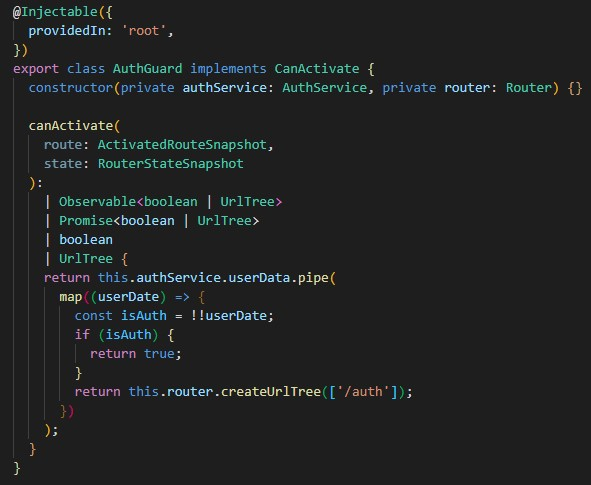
\includegraphics[width=0.5\textwidth, center]{auth-guard.jpg}
	\caption{Guard pentru autentificare}
\end{figure}

\subsection{Formularele}

Obținerea, modificarea și ștergerea datelor nu ar fi posibilă fără formularele utilizate. În cadrul acestei aplicații, pe parte de front-end a fost aleasă metoda \textit{template-driven} de implementare a formularelor (forms). Un astfel de tip folosește \textit{two-way data binding} pentru a actualiza modelul de date din componentă în timp ce au loc modificări și vice-versa \cite{angular-td-forms}.

\begin{figure}[H]
	\centering
	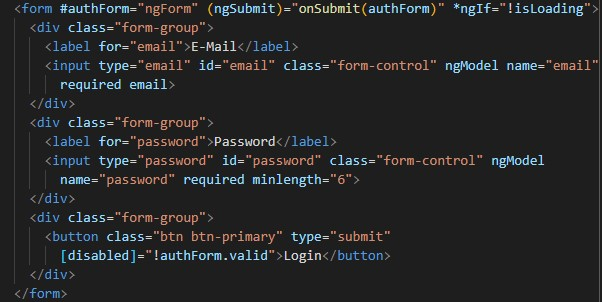
\includegraphics[width=0.6\textwidth, center]{auth-form.jpg}
	\caption{Formular de autentificare}
\end{figure}

Se poate observa cum formularul de autentificare este compus din mai multe input-uri, cel pentru email și cel pentru parolă, incluse în div-uri marcate de clasa \textit{form-group}. Fiecare input are o serie de directive specifice ce asigură restricții necesare pentru o bună experiență a utlizatorului. De exemplu, directiva \texttt{required} indică obligativitatea completării input-ului, iar \texttt{email} verifică forma corectă a email-ului.

Procesarea datelor are loc pe în codul de Typescript odată ce formularul este trimis, în acel moment fiind apelată metoda \texttt{OnSubmit} ce primește ca argument un obiect de tipul \textit{Form}.

\section{Precizări}

Versiunea de Angular utilizată este 13.

În primul rând, pentru stilizarea șabloanelor (templates) componentelor a fost folosit Bootstrap v5.2. Acest framework a permis facilitarea poziționării elementelor HTML, modificarea stilului și dimensiunilor acestora.

Căile URL necesare request-urilor către back-end au fost construite utilizând enum \textit{ApiPaths} definit în fișiserul \texttt{environment.ts}.

Pentru modelarea ușoară a obiectelor JSON în comunicarea cu back-end au fost create clase \textit{model} precum \textit{ProposalModel}, \textit{PreferenceModel} etc.
    \chapter{Back-end}

Partea de back-end a aplicației \thesistitle{} a fost implementată în framework-ul de Java Spring Boot. Această tehnologie în primul rând oferă o varietate de utilități pentru dezvoltarea web, procesare în paralel, tranazacții cu baza de date \cite{spring-boot-pros-cons}. Acesta beneficiază de un server integrat, în cazul de față este vorba de Tomcat, permițând un eventual \textit{deployment} mai ușor al aplicației. De asemenea, spre deosebire de Spring, Spring Boot nu are nevoie de o configurare XML.

În al doilea rând, acest framework permite accesul la o serie utilă de plugin-uri care permit dezvoltarea unei securități adecvate, comunicare facilă cu baza de date și simplificarea codului

Ultimul argument pentru alegerea acestei tehnologii este familiaritatea cu acesta și comunitatea extinsă de utilizatori și tutoriale.

Codul aplicației de back-end a \thesistitle{} este structurat pe straturi (layers) ce permite localizarea ușoară a claselor în funcție de rolurile acestora \cite{spring-boot-code-structure}. Există astfel module pentru \textit{controllers}, \textit{models}, \textit{repository}, \textit{service}, \textit{algorithm} etc.

\section{Inițializarea proiectului}

Datorită modului simplu și convenabil, proiectul a fost inițializat cu Spring Boot Initializr \cite{spring-boot-initializr}. Tipul proiectului este \textit{Maven}, cu versiunile de Java 11 și Spring Boot 2.7.6 pentru a fi compatibil cu versiunea de Java.

\subsection{Dependențele}

O dependență în Spring Boot poate fi comparată cu o librărie deoarece oferă anumite funcționalități. Gestionarea acestora de către programator este prin intermedul fișierului \texttt{pom.xml} (pentru un proiect Maven), odată adăugate, acestea sunt descărcate din \textit{Maven Central} (un \textit{repository} oferit de către comunitatea Maven) și stocate local în directorul \texttt{.m2} \cite{spring-boot-deps}.

Partea de back-end a proiectului \thesistitle utilizează în primul rând dependențe necesare lucrului cu baza de date. \texttt{Spring Data JPA} permite persistența datelor cu ajutorul Spring Data și Hibernate, pe când \texttt{MySQL Driver} asigură conexiunea cu baza de date MySQL. Pe lângă \texttt{Spring Web} necesară creării de servicii pentru o aplicație web, back-end-ul beneficiază și de \texttt{Spring Boot DevTools} care facilitează dezvoltarea și automatizează restart-ul aplicației. Pentru partea de securitate a aplicației a fost utilizată atât \texttt{Spring Security} pentru a crea o autentificare și o autorizare personalizate, cât și \texttt{Java JWT} pentru procesarea cheilor JWT.

Pe lângă aceste dependețe, există și altele precum \texttt{Lombok} pentru generarea codului de tipul \textit{boilerplate} (getters, setters etc.) sau \texttt{Java Faker} pentru generarea datelor entităților.

\section{Configurarea}

Fișierul \texttt{application.properties} menționat în secțiunea \textbf{4.6 Generarea datelor} conține elemente de configurare a aplicației, în special referitor la conexiunea cu baza de date. Este setat tipul bazei de date, în acest caz este MySQL, adresa la care rulează baza de date, username-ul și parola pentru conectare, precum și dialectul.

Server-ul de Tomcat este activ la adresa \texttt{\url{http://localhost:8080}} unde 8080 este portul.

Clasa \texttt{BackEndAppApplication} este cea care declanșează auto-configurarea și scanarea componentelor, pornind aplicația \cite{spring-boot-app-class}, motiv pentru care este adnotată cu \texttt{SpringBootApplication}. Tot aici este definit și metoda \texttt{passwordEncoder} adnotată cu \texttt{@Bean} (@Bean method) care descrie metoda de criptare a parolei unui utilizator cu funcția BCrypt.

\section{Arhitectura Spring Boot}

Imaginea următoare evidențiază maniera de tratare a interacțiunii cu clientul și tratarea operațiilor efectuate asupra bazei de date.

\begin{figure}[H]
	\centering
	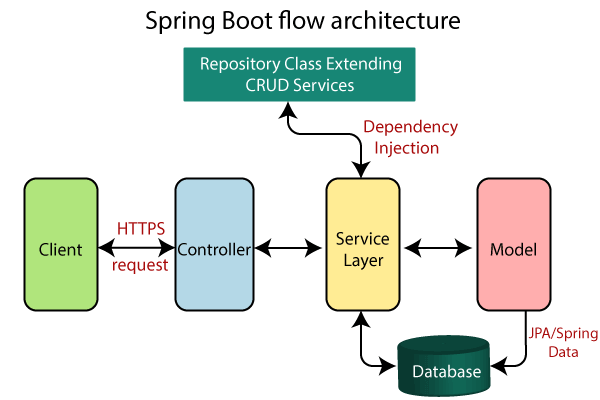
\includegraphics[width=0.8\textwidth, center]{spring-boot-architecture.png}
	\caption{Arhitectura de flux a Spring Boot}
\end{figure}

Clientul efectuează un request HTTP care este gestionat în primă instanță de \textbf{controller} care utilizează \textbf{servicii} necesare tratării request-ului. În acestea are loc logica operațiilor asupra înregistrărilor din baza de date cu ajutorul claselor \textbf{model} și prin intermediul unor clase \textbf{repository}. Informația de la client și către acesta are loc de cele mai multe ori sub forma unor obiecte DTO (Data Transfer Object) cinvertite în JSON în body-ul request-ului. Un exemplu de clasă DTO este cea a propunerilor, \texttt{ProposalDto}, ce conține strict informațiile de interes.

\begin{figure}[H]
	\centering
	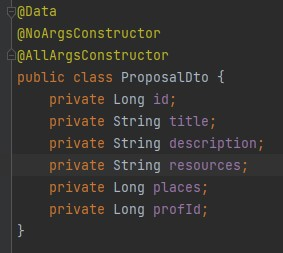
\includegraphics[width=0.4\textwidth, center]{proposaldto-class.jpg}
	\caption{Clasa ProposalDto}
\end{figure}

Aplicația de back-end poate fi considerată un \textit{REST API}. Un API este un set de definiții și protocoale pentru dezvoltarea unei aplicații de software, constituind în fapt un mediator între utilizator (în cazul de fată fiind aplicația de front-end) și resursele sau serviciile cerute într-un mod controlat și sigur \cite{rest-api}. REST (Representational State Transfer) este la rândul său un set de constrângeri arhitecturale ce trebuie respectate pentru ca un API să poată fi considerat RESTful.

Un astfel de API trebuie să urmeză în primul rând o arhitectură client-server, unde request-urile sunt gestionate prin intermediul protocolului HTTP. API-ul transferă o reprezentare a instanței unei resurse spre un anumit \textit{endpoint} (acesta include o adresă URL și identifică un canal de comunicare a resursei dintre back-end și front-end \cite{api-endpoint}), în format JSON de cele mai multe ori. De asemenea, această comunicare trebuie să fie \textit{stateless}, adică fiecare request este separat de restul și nu sunt reținute informații referitor la tranzacțiile anterioare. În al doilea rând, transferul de resurse este standardizat în ideea că acestea sunt separate de reprezentările trimise către client și manipulate de către acesta tot prin intermediul reprezentărilor \cite{rest-api}.

\section{Modelele}

Pentru a simula înregistrările dintr-o bază de date, Spring Boot dispune de posibilitatea de a defini clase ce identifică anumite entități cu ajutorul unor adnotări specifice. Spring Boot utilizează \textit{Entity Scanning} pentru a le identifica în loc de un fișier special cum ar fi \texttt{persistence.xml} în Spring. Clasele luate în considerare sunt cele adnotate cu \texttt{Entity}, \texttt{Embeddable} sau \texttt{MappedSuperclass} \cite{spring-boot-docs}.

Se observă de exemplu clasa \texttt{User}.

\begin{figure}[H]
	\centering
	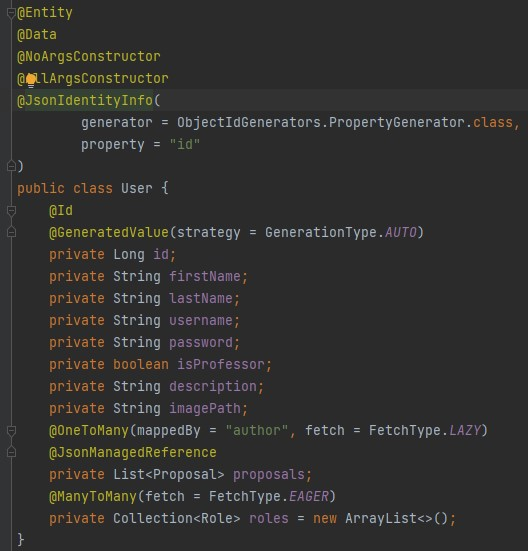
\includegraphics[width=0.6\textwidth, center]{user-class.jpg}
	\caption{Clasa User}
\end{figure}

Proprietățile acestei clase identifică câmpurile, identificate de numele lor, ale tabelei \texttt{user} din baza de date, iar tipul lor este conform reprezentării lor. Id-ul este generat automat cu ajutorul unei valori reținute în tabela \texttt{hibernate\_sequence} creată de framework-ul Hibernate, fiind de asemenea adnotată cu \texttt{@Id} pentru a sublinia că această proprietate reprezintă cheie primară.

Un utilizator de tipul profesor are o listă de propuneri (proposals, care sunt proiecte ori tematici), relația dintre tabela \texttt{user} și \texttt{proposal} prin intermediul cheilor străine (foregin keys) fiind specificată prin adnotarea \texttt{@OneToMany}. Opțiunea de \texttt{FetchType.LAZY} permite încărcarea mai rapidă a utilizatorului deoarece propunerile sale sunt instanțiate numai în cazul în care este nevoie. Fiecare utilizator are de altfel o colecție de roluri care pot fi \texttt{ROLE\_USER} în mod normal sau \texttt{ROLE\_ADMIN} și indică drepturile sale în aplicație.

Există și situația ca id-ul unei entități, precum cea a acordului, să fie compus, deoarece la nivelul reprezentării în tabela \texttt{accord}, o înregistrare este identificată prin id-urile studentului și profesorului care au hotărât colaborarea în realizarea unui anumit proiect. În consecință, a fost necesară crearea unei noi clase \texttt{AccordKey} care să simuleze cheia primară compusă și adnotarea proprietății cu \texttt{@EmbeddedId}.

\section{Clasele \textit{repository}}

Pentru fiecare entitate modelată în cadrul aplicației există o clasă \textit{repository} care reprezintă un mecanism de stocare, căutare și modificare a informațiilor din baza de date. Aceasta implementează interfața generică \texttt{JpaRepository} (Java Persistence API) care furnizeză o serie de metode CRUD (Create Read Update Delete) pentru accesarea datelor. Există posibilitatea de definirea a unor metode particulare prin cuvinte cheie care ajută la generarea automată a interogărilor SQL, fiind un mod clar și facil de efectuare a operațiilor \cite{jpa-repository}. Astfel de clase descriu nivelul de acces al datelor (Data Acces Layer)

\begin{figure}[H]
	\centering
	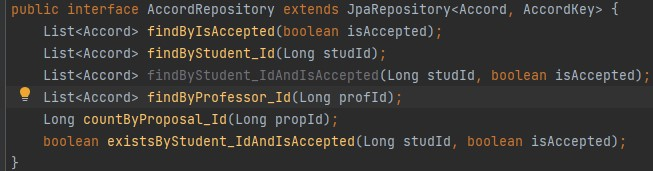
\includegraphics[width=0.8\textwidth, center]{accord-repository.jpg}
	\caption{Repository pentru un acord}
\end{figure}

Clasa \texttt{AccordRepository} conține de exemplu patru metode de căutare a acordurilor, în funcție de diferiți parametri. Metodele pot returna și dacă există o numită înregistrare, precum și numărul de anumite înregistrări. Datele sunt salvate sau actualizate cu metoda \texttt{save} ce primește ca argument un obiect entitate, în cazul în care id-ul este null, este introdusă o nouă înregistrare, altfel este modificată cea cu id-ul respectiv.

\section{Serviciile}

Aplicația dispune pentru entități de interfețe servicii corespunzătoare ce descriu metode de manipulare a datelor respective, implementate mai departe de clase ce trebuie adnotate cu \texttt{@Service} și care crează funcționalitățile necesare, reprezintă astfel teoretic nivelul serviciilor.

Serviciile utilizează clase \textit{repository} după cum este prezentat în figura următoare.

\begin{figure}[H]
	\centering
	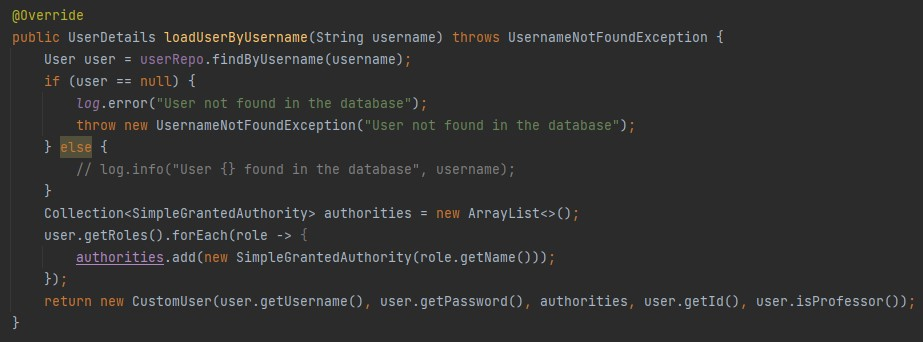
\includegraphics[width=0.8\textwidth, center]{user-service-load-method.jpg}
	\caption{Metodă de obținere a utilizatorului după username}
\end{figure}

Aceasta obține un obiect de tipul \texttt{User} cu un username dat și în plus rolurile acestuia, fiind convertit ulterior în \texttt{CustomUser} pentru verificarea și autorizarea utilizatorului autentificat în contextul aplicației.

\section{Controlerele (Controllers)}

Într-un final, cel de-al treilea nivel, de prezentare (presentation layer), este constituit de controlere care efectuează comunicarea cu partea de front-end și ale căror clase sunt adnotate cu \texttt{RestController}. Metodele descriu tratarea request-urilor HTTP cu ajutorul diferitelor servicii.

\begin{figure}[H]
	\centering
	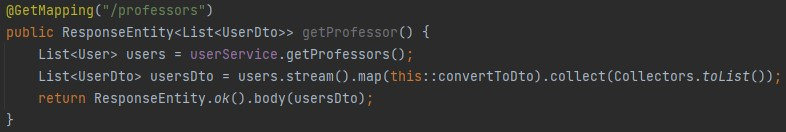
\includegraphics[width=1\textwidth, center]{user-controller-get-method.jpg}
	\caption{Metodă de trimitere a tuturor profesorilor}
\end{figure}

\begin{figure}[H]
	\centering
	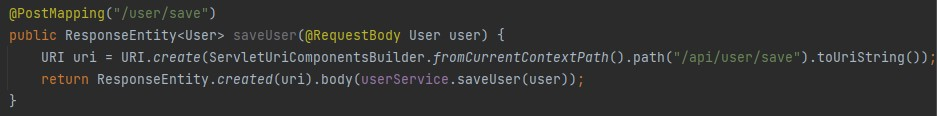
\includegraphics[width=1\textwidth, center]{user-controller-post-method.jpg}
	\caption{Metodă de salvare a unui utilizator}
\end{figure}

În cazul clasei \texttt{UserController}, metoda \texttt{getProfessors} este apelată de fiecare dată când este primit un request de tipul GET la endpoint-ul \texttt{"/professors"}, lucru evidențiat de adnotarea premergătoare definiției. Răspunsul HTTP este reprezentat de un obiect de tipul \texttt{ResponseEntity} cu \textit{status code} 200 (cerere efectuată cu succes) și având în \textit{body} o listă de obiecte de tipul \texttt{UserDto}, după cum a fost precizat anterior.

Metoda \texttt{saveUser} primește ca parametru un utilizator transmis prin body-ul request-ului POST, lucru ce trebuie specificat prin adnotarea \texttt{@RequestBody}.

\section{Securitatea}

Securitatea aplicației este dezvoltată de pachetul \texttt{security} care conține în principal clasa \texttt{SecurityConfig} ce extinde clasa abstractă \texttt{WebSecurityConfigurerAdapter} și este adnotată cu \texttt{Configuration} și \texttt{EnableWebSecurity}. Aceasta suprascrie metoda \texttt{configure} care indică maniera de tratare a utilizatorului ce interacționează cu aplicația.

\begin{figure}[H]
	\centering
	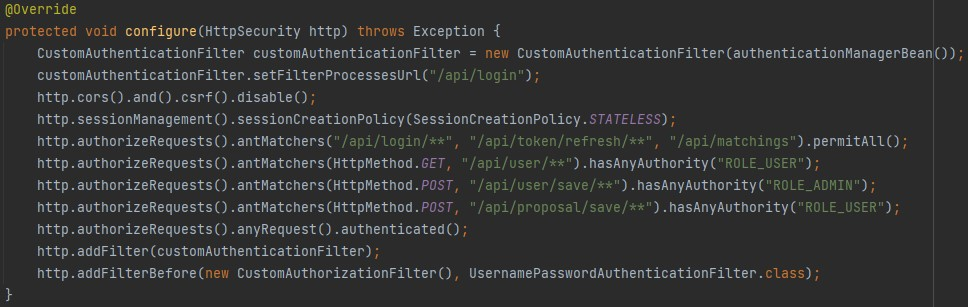
\includegraphics[width=1\textwidth, center]{security-configure-method.jpg}
	\caption{Metodă de configurare a securității}
\end{figure}

Metoda primește ca parametru o variabilă \texttt{http} de tipul \texttt{HttpSecurity} și care permite configurarea contextului abordat. Utilizând un sistem bazat pe chei JWT (JSON Web Token), aplicația de back-end nu trebuie să creeze o sesiune pentru fiecare utilizator.

JWT este un standard care definește un mod compact de trasmitere sigură a informațiilor între aplicații sub forma unor obiecte JSON, putând fi considerată o semnătură digitală a utilizatorului. Un astfel de token are trei părți separate de punct: header, payload și semnătură. Header-ul conține tipul token-ului, adică JWT, și algoritmul folosit pentru semnarea acestuia, aplicația \thesistitle utilizează \textit{HMAC256}. Payload-ul conține pretențiile (claims) cum ar fi rolurile deținute, dacă utilizatorul este profesor sau nu și altele. Semnătura este obținută prin criptarea primelor două părți cu algoritmul specificat și un șir de caractere secret știut doar de către back-end \cite{jwt}. Fiecare token are un termen de validitate pentru a indica perioada în care utilizatorul este autentificat.

De asemenea, request-urile din partea clientului sunt autorizate în funcție de anumite filtre, implementându-se în acest scop unul pentru autentificare în primă instanță și unul pentru autorizare.

\subsection{Autentificarea}

Autentificarea este verificarea identității unui utilizator, în acest caz find realizată într-un mod clasic cu ajutorul username-ului și parolei. Utilizatorul furnizeză credențialele sale care sunt verificate pe partea de back-end și sunt luate măsuri în funcție de validitatea acestora \cite{spring-security}.

Verificarea este asigurată de un filtru de autentificare.

\begin{figure}[H]
	\centering
	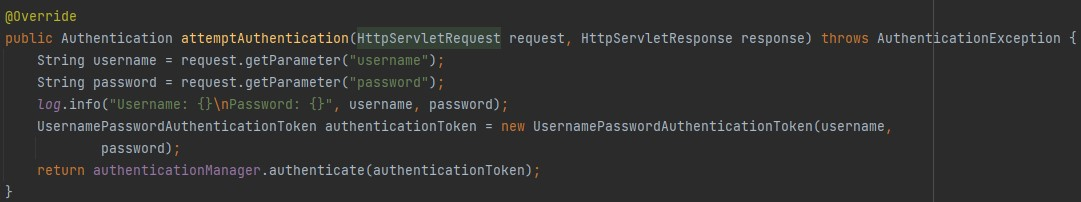
\includegraphics[width=1\textwidth, center]{attempt-authentication-method.jpg}
	\caption{Tentativă de autentificare}
\end{figure}

Atunci când un utilizator dorește acces la aplicație, în metoda descrisă mai sus este informată proporietatea \texttt{authenticationManager} de datele utilizatorului și încercă autentificarea acestuia.

\begin{figure}[H]
	\centering
	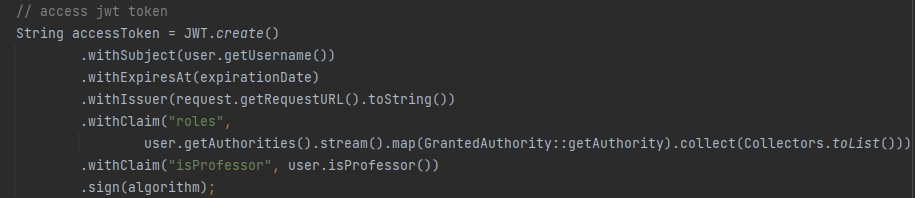
\includegraphics[width=1\textwidth, center]{successful-authentication-method-snippet.jpg}
	\caption{Autentificare cu succes}
\end{figure}

În cazul în care este autentificat cu succes, este creată cheia de acces, denumită \texttt{accessToken}, în metoda suprascrisă \texttt{successfulAuthentication}. Token-ul va conține informații despre username-ul persoanei, termenul de valabilitate, rolurile și tipul acesteia. Rezultatul este trimis către client sub formă de JSON. Această cheie JWT va fi folosită în toate request-urile viitoare ale utilizatorului pentru confirmare identității acesteia.

\subsection{Autorizarea}

Autorizarea este deciderea dacă o anumită persoană are permisiunea de a accesa o anumită resursă și este realizată în funcție de rolurile acesteia. Un administrator va avea de aceea un număr extins de drepturi cum ar fi adăugarea unui nou utilizator, acțiune pe care un cont doar cu ROLE\_USER nu o poate face. Modalitatea de autorizarea este restricționarea anumitor URL-uri în funcție de permisiuni \cite{spring-security}.

În consecință, fiecare utilizator este obligat ca, odată ce este autentificat, să poată fi identificat și autorizat înaintea de executarea request-urilor efectuate. După autentificarea cu succes a sa, utilizatorul primește un JWT (JSON Web Token), un șir de caractere ce conține criptat informații specifice cum ar fi username-ul, tipul de utilizator (profesor sau student) și permisiunile sale (ROLE\_USER, ROLE\_ADMIN).

\begin{figure}[H]
	\centering
	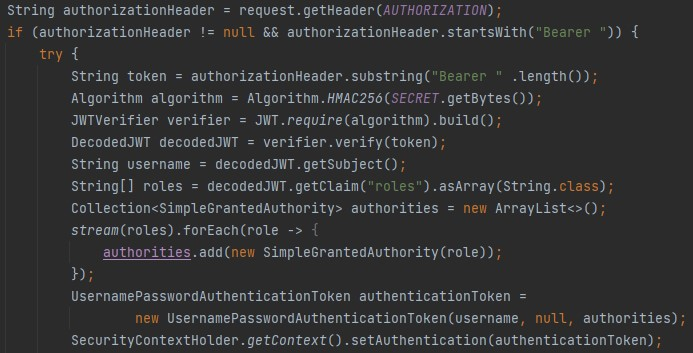
\includegraphics[width=1\textwidth, center]{authorization-filter-snippet.jpg}
	\caption{Autorizarea în \texttt{CustomAuthorizationFilter}}
\end{figure}

În filtrul de autorizare, este verificată validitatea requset-ului primit. Acesta trebuie să conțină un header \textit{Authorization} cu valoarea token-ului unic precedat de șirul de caractere "Bearer ". Cheia JWT este decriptată și este decisă acordarea permisiunii pentru reqest-ul respectiv. Dacă nu sunt îndeplinite condițiile adecvate, este trimis un răspun cu status code 401, \textit{Unauthorized}, sau 403, \textit{Forbidden}.
\\~\\
\indent După definirea celor două filtre cu responsabilitățile specifice, acestea sunt ordonate în mod logic pantru verificarea datelor și sunt descrise condițiile de validitate pentru rutele corespunzătoare request-urilor.

Există pe lângă cele două mecanisme menționate anterior un filtru care gestionează verificările CORS (Cross-Origin Resource Sharing) în care este specificată adresa de origine a aplicației de front-end, a clientului. Server-ul primește din partea browser-ului înainte de procesarea fiecărui request un \textit{preflight request} care verifică permisiunile pentru anumite metode HTTP. În consecință, metoda @Bean \texttt{corsConfigurationSource} din clasa \texttt{SecurityConfig} marchează adresa de origine \texttt{\url{http://localhost:4200}} a front-end-ului ca fiind de încredere și permite efectuarea request-urilor provenind de la acesta.
    \chapter{Algoritmul de repartizare}

Problema pe care își propune această aplicație să o rezolve este o instanță a problemei asignării sau problema atribuirii (\textit{assignment problem}). Este de precizat că cele două nume vor fi folosite interschimbabil în secțiunile următoare. În cazul de față, instanța este reprezentată de o mulțime de studenți, fiecare cu o ordonare a unor preferințe, și o mulțime a propunerilor profesorilor (proiecte sau tematici generale). Cerința este repartizarea optimă a propunerilor către studenți în funcție de preferințele acestora.

În literatura de specialitatea au fost descriși și dezvoltați diverși algoritmi de rezolvare a unei astfel de instanțe a problemei atribuirii. Algoritmul implementat de aplicația \thesistitle{} este unul din clasa de algoritmi de licitație (\textit{auction algorithms}), descris în lucrarea "Assignment Problem with Constraints" scrisă de către Ulrich Bauer, Facultatea de Informatică a Universității Tehcnice din München, 2005. Pentru a descrie coerent și cât mai clar logica acestui algoritm, în secțiunile următoare vor fi descrise problema atribuirii și similitudinile acesteia cu o problemă de flux, conceptele matematice ale algoritmilor propuși pentru rezolvare și pașii algoritmului implementat pentru instanța prezentă.

\section{Problema asignării (atribuirii)}

Problema simetrică a asignării constă în două mulțimi $X$ și $Y$ de dimensiuni egale, o mulțime $E \subseteq X \times Y$ și o funcție de cost $c_{xy}$ pentru oricare pereche posibilă $(x, y) \in E$. Scopul este cuplarea oricărui element din $X$ cu un element din $Y$ ca la final costul total să fie minim \cite{assignment}.

În contextul grafurilor, această problemă poate fi redusă la problema fluxului de cost minim într-un  graf bipartit $G=((X \bigcup Y,\ E)$ cu o funcție de cost $c_{xy},\ (x, y) \in E$, și capacitatea $u_{xy} = 1, \forall (x, y) \in E$. 

Expresia matematică a problemei \cite[p.~6]{assignment} este 
\[ minimizarea \sum_{(i, j) \in E} c_{ij} x_{ij} \]
astfel încât
\[ \sum_{j:(i, j) \in E} x_{ij} = 1, \forall i \in X, \]
\[ \sum_{i:(i, j) \in E} x_{ij} = 1, \forall j \in Y, \]
\[ x_{ij} \geq 0, \forall (i, j) \in E \].

Variabila $x_{ij}$ indică câtă unități de flux sunt trimise pe muchia $(i, j)$.

Cu toate acestea, problema repartizării fiecărui student o teză de licență în funcție de preferințele sale este o problemă asimetrică deoarece numărul de propuneri, $|Y|$, este mai mare sau egal decât numărul de studenți (trebuie să fie măcar egal pentru a putea atribui fiecărui student o lucrare). La final, o soluția determinată se va afla în variabila $x_{ij}$ unde dacă $x_{ij} = 1$, atunci studentului $i$ îi este repartizată propunerea $j$ din totalul de propuneri al tuturor profesorilor.

Important de precizat este că în acest caz, rating-ul total al preferințelor satisfăcute trebuie maximizat. De aceea, este realizată o normalizare în primă instanță pentru a transforma rating-urile în costuri, prin calcularea $c_{ij} = 101 - rating_{ij},\: rating_{ij} \in \mathbb{N} \cap [1, 100],\: \forall (i, j) \in E$.

\section{Algoritmul de licitație}

Algoritmul de licitație este o metodă intuitivă ce rezolvă problema clasică a atribuirii (asignării), reușind de asemenea să depășească în performanță algoritmi similari, fiind în același timp potrivit pentru calculul în paralel \cite[p.~1]{auction}. Acest algoritm a fost propus de matematicianul Dimitri Bertsekas și este în sine o metodă euristică aplicată algoritmului \textit{push/relabel} pentru a îmbunătăți rezultatele practice \cite[p.~24]{assignment}, având în mod similar o complexitate de $\mathcal{O}(n m \log(n C))$ unde $n$ este numărul total de noduri ($|X|+|Y|$), $m$ este numărul de muchii $|E|$, iar $C = max_{(i, j)}\{c_{ij}\}$ este maximul costurilor. 

Algoritmul de licitație poate fi descris ca o licitație în viața reală. Elementele din mulțimea $X$, studenții, licitează pentru elementele din $Y$, lucrările propuse de profesori. Pentru un student $i$, propunerea $j$ este cea mai benfică dacă suma costului $c_{ij}$ și prețul $\pi(j)$ este minim, iar o propunere este atribuită studentului cu cea mai bună ofertă\cite{assignment}. Funcția $\pi$ este utilizată în pasul de reetichetare (\textit{relabel}) a unei propuneri.

Pentru a permite finalizarea algoritmului, prețurile $\pi$ trebuie să crească cu o valoare $\epsilon$. Mai mult decât atât, Bertsekas a fost primul care a propus scalarea prin $\epsilon$ (\textit{$\epsilon$-scaling}) pentru a îmbunătăți performanța algoritmului în cazul instanțelor unde numărul de obiecte din $Y$ licitate este mai mic. În cazul în care $\epsilon$ este prea mic, poate apărea un "război al prețurilor" când este nevoie de o creștere mai substanțială a prețurilor, deci un număr mare de iterații, până anumiți studenți găsesc propuneri mai profitabile decât cele licitate. Soluția este execuția algoritmului începând cu $\epsilon$ inițializat cu cel mai mare cost al preferințelor ($C$) și scăderea treptată a acestuia de la o iterație la alta.

Algoritmul de licitație poate fi corelat cu unul de calculare a unui flux de cost minim, cu un graf $G=(X \cup Y, E)$ unde $X$ reprezintă studenții, iar $Y$ propunerile. Este definită o nouă variabilă 
$c_{ij}^\pi$ numită costul redus al muchiei $(i, j)$ din graful $G=(V, E)$ în raport cu funcția de preț $\pi: V \rightarrow \mathbb{R}_+$,\; $c_{ij}^\pi = c_{ij} - \pi(i) + \pi(j)$.

Un pas de licitație este numit \textit{double-push} deoarece este echivalent cu operațiile \textit{push} și \textit{relabel}. Când un student $x$ licitează pentru un proiect $y$, este efectuat un flux pe muchia $(x, y)$. Dacă $y$ a fost deja asigant unui $x'$, $y$ transmite flux către $x'$ deoarece are un exces pozitiv.

\subsection{Algoritmul de licitație pentru problema asimetrică a asignării}

În cazul problemei asimetrice de asignare, $|X| \leq |Y|$ și trebuie determinat care dintre muchii trebuie luate în calcul. Se poate întâmpla ca după o iterație, prețul unui element din $Y$ poate deveni prea mare și poate rămâne neasignat în iterația următoare, deși ar putea fi preferat de către un student. În cazul problemei simetrice, fiecare $y \in Y$ este asignat.

O primă abordare este transformarea problemei asimetrice într-una simetrică prin introducerea unor $|Y| - |X|$ noduri "virtuale" în mulțimea $X$, fiecare dintre ele conectat la toate nodurile din $Y$  cu câte un cost 0. Acest lucru poate rezulta însă la un graf dens din punct de vedere al muchiilor.

O altă abordare, utilizată și în proiectul de față, este utilizarea unui arbore binar (\textit{binary heap}). De fiecare dată când este reetichetat (\textit{relabeled}) un nod care nu se află în heap, este introdus în heap și eliminat din acesta nodul cu cel mai mic preț. Dacă acest nod este atribuit, fluxul pe muchia respectivă devine 0. Utilizând un arbore binar, reetichetarea nodului are loc cu o complexitate de $\mathcal{O}(\log(|X|)$, iar accesarea nodului cu cel mai mic preț este imediată deoarece se află în vârf. Complexitatea generală a algoritmului crește la $\mathcal{O}(n m \log(n C) \log(|X|))$, care nu afectează mult însă performanța algoritmului.

\section{Pseudocod}

Algoritmii următori scriși în pseudocod și utilizați de aplicație au fost descriși în lucrarea menționată anterior, \textit{Constrained Assignment} \cite{assignment}.

\subsection{Funcția \textit{doublePush} cu arbore binar (heap)}

\begin{algorithm}
	\caption{$doublePush(i)$}
	\begin{algorithmic}[1]
		\State Fie $(i, j)$ și $(i, k)$ muchii astfel încât $c_{ij}^\pi$ să fie minim și $c_{ik}^\pi$ al doilea cel mai mic
		\State $x_{ij} \gets 1$ //push 
		\If{$j \notin H$} // $H$ este arborele binar (heap)
			\State $H.put(\pi(j),\ j)$ // j este introdus în heap cu cheia prețul său actual
			\If{$|X| > H.size()$}
				\State $g \gets H.min()$
				\State $H.removeMin()$
				\If{$\exists f \in X$, $x_{fg} = 1$} // propunerea g este deja asignată unui student f
					\State $x_{fg} \gets 0$ // push
				\EndIf
			\EndIf
		\EndIf
		\If{$\exists h \in X$, $h \neq i$ și $x_{hj} = 1$} // propunerea j era deja atribuită unui alt student h
			\State $x_{hj} \gets 0$ // push
		\EndIf
		\State $\pi(j) \gets \pi(k) + c_{ik} - c_{ij} + \epsilon$ // relabel
	\end{algorithmic}
\end{algorithm}

\subsection{Funcția \textit{refine} de îmbunătățire a rezultatului}

\begin{algorithm}
	\caption{$refine()$}
	\begin{algorithmic}[1]
		\State $\epsilon \gets \epsilon / \alpha$ // $\alpha$ este o constantă aleasă în mod euristic
		\ForAll{$(i, j) \in E$}
			\State $x_{ij} \gets 0$
		\EndFor
		\While{$\exists i \in X$, $i$ neasignat}
			\State $doublePush(i)$
		\EndWhile
	\end{algorithmic}
\end{algorithm}

\subsection{Algoritmul de licitație pentru asignare}

\begin{algorithm}
	\caption{$solve()$}
	\begin{algorithmic}[1]
		\State $\epsilon \gets max_{(i, j) \in E}\{c_{ij}\}$
		\ForAll{$j \in Y$} //inițializează prețul tuturor propunerilor cu 0
			\State $\pi(j) \gets 0$
		\EndFor
		\While{$\epsilon \geq 1 / n$}
			\State $refine()$
		\EndWhile
		\State return $x$
	\end{algorithmic}
\end{algorithm}

\section{Implementare}

Implementarea algoritmului prezentat anterior a avut loc în limbajul Java pentru a putea fi folosit în cadrul unei aplicații de Spring Boot. A fost creată în mod special clasa \textit{Edge} pentru a modela muchiile dintre cele două mulțimi $X$ a studenților și $Y$ a propunerilor, mai precis preferințele studenților. Câmpul \textbf{start} indică indicele studentului și câmpul \textbf{end} indică indicele propunerii preferate.

\begin{figure}[H]
	\centering
	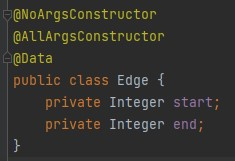
\includegraphics[width=0.5\textwidth, center]{edge-class.jpg}
	\caption{Clasa Edge}
\end{figure}

\subsection{Preprocesarea datelor}

Înainte de efectuarea algoritmului, este nevoie de operații de preprocesare pentru a converti obiectele primite de la baza de date (studenții, propunerile, preferințele) în variabile de input adecvate. Pentru acest lucru a fost creată clasa \textit{Convertor} care utilizează patru servicii, \texttt{accordService}, \texttt{preferenceService}, \texttt{proposalService} și \texttt{userService}, pentru a accesa înregistrările din baza de date, reținându-se în două liste \texttt{studIds} și \texttt{propIds} id-urile studenților (students) și propunerilor (proposals). Sunt eliminate id-urile care se află într-un acorduri acceptate, adică cele care au câmpul $\texttt{isAccepted} = true$.

Algoritmul este nevoit să primească listele $X$ și $Y$ sub formă de indecși ale elementelor în listele \texttt{studIds} \texttt{propIds}, iar nu id-urile în mod direct, deoarece propunerile pot fi de două feluri: proiect (project) sau tematică (topic). Tematicile pot avea un număr de locuri disponibile mai mare de 1, de aceea în \texttt{propIds} se adaugă duplicate ale aceluiași id câte locuri sunt disponibile.

Indecșii id-urilor studenților sunt reținute într-o variabilă \texttt{studIndices} de tipul \texttt{HashMap<Long, Integer>} unde cheile sunt id-urile, iar valorile sunt indecșii în lista de id-uri. Similar, indecșii propunerilor sunt reținuții în variabila \texttt{propIndices} de tipul \texttt{HashMap<Long, List<Integer>>} de această dată deoarece un id de propunere poate avea mai multe duplicate în listă.

După aceste convertiri, este calculată o variabilă $c$ a costurilor (similară modelului teoretic) de tipul \texttt{HashMap<Edge, Double>} unde cheile sunt muchiile (preferințele), iar valorile acestora sunt costurile. Un cost se calculează astfel: preferințele unui student sunt ordonate descrescător, teza de licență cea mai favorabilă primind costul 1.0, iar două propuneri cu același rating primind același cost.

\subsection{Algoritmul}

Algoritmul este modelat de clasa \textit{AssignAlgorithm} ce este inițializat cu variabilele $n$ numărul de studenți, $m$ numărul de propuneri, $c$ variabila costurilor. Clasa dispune de metodele similare algoritmilor prezentați anterior în pseudocod.

În metoda \textit{solve()} este inițializată o listă \texttt{unassigned} cu toți studenții neatribuiți. Se inițializează variabila $eps$ cu cel mai mare cost din $c$ și variabila $pi$ este setată pe valoarea 0 pentru toate propunerile. Cât timp $eps$ nu depășește pragul $alpha / (n + m)$ se execută metoda \textit{refine()}.

Metoda \textit{refine()} reinițializează variabila soluție $x$ cu 0 pe fiecare muchie. Se alege în mod aleatoriu un student neasignat și se execută metoda \textit{doublePushHeap(i)}.

\begin{figure}[H]
	\centering
	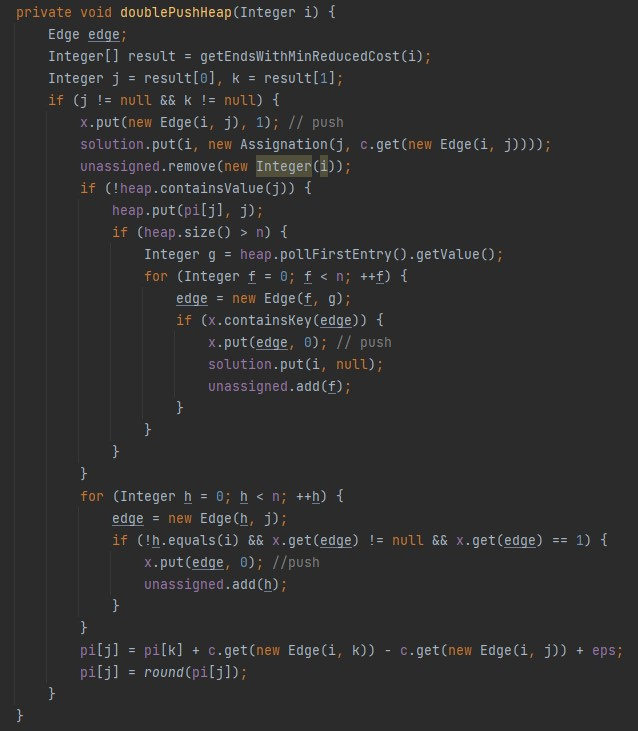
\includegraphics[width=0.7\textwidth, center]{double-push-method.jpg}
	\caption{Metoda \textit{doublePushHeap}}
\end{figure}

Este definită variabila locală \texttt{result} ca un tablou de două poziții. Poziția \texttt{result[0]} conține $j$, iar, \texttt{result[1]} conține $k$, unde $(i, j)$ este muchia cu cel mai mic cost redus și $(i, k)$ muchia cu al doilea cel mai mic cost redus. Variabila \texttt{heap} a fost declarată de tipul \texttt{TreeMap<Double, Integer>} unde cheile sunt prețurile propunerilor (\texttt{$\pi[j]$}) și valorile sunt indecșii. Acest lucru permite ordonarea propunerilor asignate în funcție de prețul acestora, de asemenea accesarea propunerii (elementului $j \in Y$) cu prețul $\pi(j)$ minim are loc în $\mathbb{O}(1)$.

Orice alt student $h$ asignat anterior propunerii $j$ este marcat ca fiind neasignat (push step). În contextul problemei fluxului într-un graf bipartit, fluxul dinspre studentul $i$ spre propunerea $j$ este setat pe 0.

\begin{figure}[H]
	\centering
	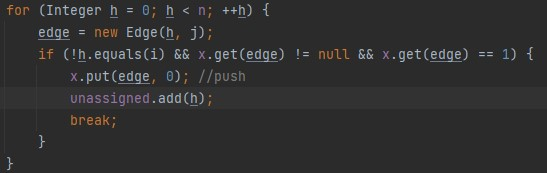
\includegraphics[width=1\textwidth, center]{push-step.jpg}
	\caption{Pasul de push}
\end{figure}

Pasul final este cel de reetichetare (relabel step) observat în imaginea următoare.

\begin{figure}[H]
	\centering
	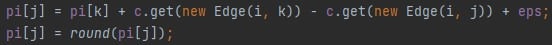
\includegraphics[width=1\textwidth, center]{relabel-step.jpg}
	\caption{Pasul de relabel}
\end{figure}

\subsection{Procesarea rezultatului}

Soluția constă într-o variabilă de tipul \texttt{Map<Integer, Assignation>} cu cheile reprezentând indecșii studenților în lista \texttt{studIds}. Valorile sunt de tipul \texttt{Assignation} ce conține câmpul \texttt{end} ce reprezintă indexul propunerii atribuite în lista \texttt{propIds} și câmpul \texttt{cost} ce are calculat calitatea preferinței satisfăcute. Acest lucru permite accesarea rapidă a soluției pentru un student $i$ și construirii rezultatului total.

\begin{figure}[H]
	\centering
	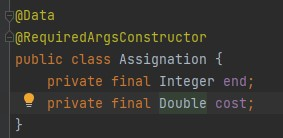
\includegraphics[width=0.6\textwidth, center]{assignation-type.jpg}
	\caption{Tipul Assignation}
\end{figure}

La finalul execuției algoritmului, există posibilitatea ca un număr de studenți să nu aibă proiecte atribuite în cazul în care aceștia nu au avut un număr de preferințe îndeajuns de mare. Dacă există o astfel de situație, se alege în mod aleatoriu un student dintre aceștia și îi este asignată o propunere dintre cele care nu au fost încă luate până când toți studenții sunt repartizați.

Rezultatul final este alcătuit în primul rând din studenții care au stabilit acorduri cu profesori pentru anumite proiecte, repartizările calculate de algoritm și repartizările ulterioare ale studenților neatribuiți.

Din punct de vedere tehnic, rezultatul transmis către front-end prin intermediul unui request de tipul GET este o listă de obiecte de tipul \texttt{MatchingDto} (DTO = Data Transfer Object).

\begin{figure}[H]
	\centering
	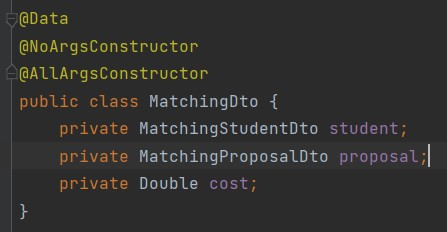
\includegraphics[width=0.7\textwidth, center]{matchingdto-class.jpg}
	\caption{Clasa MatchingDto}
\end{figure}

\begin{figure}
\centering
	\begin{minipage}{0.5\textwidth}
		\centering
		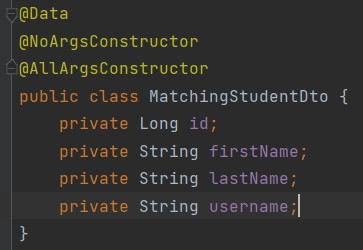
\includegraphics[width=1\linewidth]{matchingstudentdto-class.jpg}
		\caption{Clasa MatchingStudentDto}
	\end{minipage}%
	\begin{minipage}{0.5\textwidth}
		\centering
		\includegraphics[width=1\linewidth]{matchingproposaldto-class.jpg}
		\caption{Clasa MatchingProposalDto}
	\end{minipage}
\end{figure}

\section{Precizări}

Variabila \texttt{pi} conține valori reale, dar a fost considerat că o precizie de două variabile este de ajuns pentru efectuarea algoritmului. Pentru trunchierea valorilor, a fost implementată o metodă statică \texttt{round(double value)} care aproximează superior prețurile calculate.

\begin{figure}[H]
	\centering
	\includegraphics[width=1\textwidth, center]{round-method.jpg}
	\caption{Rotunjirea prețurilor}
\end{figure}

Constanta \texttt{alpha} a fost inițializată cu valoarea 10, urmând recomandările menționate în lucrarea \textit{Constrained Assignment} \cite[p.~46]{assignment}.

Variabila \texttt{eps} are valorea inițială egală cu cel mai mare cost dintre muchiile existente.

    \chapter{Indicații de utilizare}

Amet venenatis urna cursus eget. Quam vulputate dignissim suspendisse in est ante. Proin nibh nisl condimentum id. Egestas maecenas pharetra convallis posuere morbi. Risus viverra adipiscing at in. Vulputate eu scelerisque felis imperdiet. Cras adipiscing enim eu turpis egestas pretium aenean pharetra. In aliquam sem fringilla ut morbi tincidunt augue. Montes nascetur ridiculus mus mauris. Viverra accumsan in nisl nisi scelerisque eu ultrices vitae. In nibh mauris cursus mattis molestie a iaculis. Interdum consectetur libero id faucibus nisl tincidunt eget. Gravida in fermentum et sollicitudin ac orci. Suscipit adipiscing bibendum est ultricies. Etiam non quam lacus suspendisse. Leo urna molestie at elementum eu facilisis sed odio morbi. Egestas congue quisque egestas diam in arcu cursus. Amet consectetur adipiscing elit ut aliquam purus.

Eros donec ac odio tempor. Facilisi morbi tempus iaculis urna id volutpat. Faucibus in ornare quam viverra orci sagittis eu. Amet tellus cras adipiscing enim eu turpis egestas. Integer feugiat scelerisque varius morbi. Platea dictumst vestibulum rhoncus est pellentesque elit ullamcorper dignissim. Bibendum arcu vitae elementum curabitur. Eu nisl nunc mi ipsum faucibus. Id aliquet lectus proin nibh nisl condimentum id venenatis a. Cras adipiscing enim eu turpis egestas pretium. Quisque non tellus orci ac auctor augue mauris augue. Malesuada pellentesque elit eget gravida cum. Ut lectus arcu bibendum at. Massa id neque aliquam vestibulum morbi blandit. Posuere ac ut consequat semper viverra nam. Viverra adipiscing at in tellus integer feugiat scelerisque varius morbi. Morbi enim nunc faucibus a pellentesque sit amet porttitor eget. Eu feugiat pretium nibh ipsum consequat nisl vel. Nisl purus in mollis nunc sed.

Elementum sagittis vitae et leo duis ut diam quam nulla. Purus sit amet volutpat consequat mauris nunc. Tincidunt augue interdum velit euismod in pellentesque massa. Nunc sed augue lacus viverra vitae congue. Porttitor leo a diam sollicitudin. Faucibus pulvinar elementum integer enim. Adipiscing bibendum est ultricies integer quis auctor elit. Blandit aliquam etiam erat velit scelerisque in. A iaculis at erat pellentesque adipiscing commodo elit at. Erat nam at lectus urna duis. Consequat ac felis donec et. Fermentum posuere urna nec tincidunt praesent semper feugiat nibh sed. Proin gravida hendrerit lectus a. Pretium viverra suspendisse potenti nullam ac tortor vitae purus. Arcu cursus euismod quis viverra nibh cras pulvinar mattis. Gravida arcu ac tortor dignissim convallis aenean. Quam nulla porttitor massa id neque aliquam vestibulum morbi. Sed viverra ipsum nunc aliquet. Quis enim lobortis scelerisque fermentum dui faucibus in.
    
    \chapter*{Concluzii} 
\addcontentsline{toc}{chapter}{Concluzii}

Aplicația \thesistitle{} propune să rezolve problema des întâlnită în facultăți de a repartiza studenții la profesorii de licență, mai precis de a atribui tezele propuse studenților ținând cont de preferințele lor. Într-un final, scopul principal este de a oferi șansa viitorilor absolvenți de a realiza o lucrare finală pe măsura aptitudinilor cumulate pe parcursul anilor de studenție, dar și în funcție de înclinațiile lor spre o anumită specializare. Mai mult decât atât, aplicația oferă posibilitatea unei cercetări riguroase de către student a proiectelor propuse prin centralizarea acestora și opțiunea de a conveni cu un profesor asupra unei propuneri favorabile, sub forma unui acord.

Dezvoltarea acestei aplicații a oferit prilejul cercetării mai amănunțite a tehnologiilor utilizate și dezvoltării abilităților în crearea de soluții software. Aplicația prezintă astfel interes în modul de adaptare a interfeței în funcție de utilizator și în același timp adoptarea unui design simplist și intuitiv. Partea de back-end prezintă o implementare personalizată a mecanismului de securitate adaptat unui context special, de uz intern.

Pe lângă aceste aspecte, urmând a rezolva problema de față, au fost cercetați mai mulți algoritmi potențiali, alegându-se într-un final un algoritm de atribuire prin double-push cu heap. Una dintre provocări a fost adaptarea datelor problemei la cele de intrare (input) și optimizarea prelucrării informațiilor de la baza de date. De asemenea, implementarea conceptelor teoretice descrise în Java constă un alt interes prin modularizarea și particularitățile codului.

\section*{Posibile dezvoltări viitoare}

Aplicația prezintă o serie de direcții de dezvoltare în viitor, prezentând un potențial de a deveni după anumite îmbunătățiri și modificări o aplicație utilitară robustă în contextul intern al facultății.

O primă idee de dezvoltare este implementarea unor noi algoritmi adaptați datelor de intrare în urma cercetării performanțelor acestora. O altă idee este implementarea unui sistem de preferințe și pentru profesori care vor putea nu numai încheia acorduri pentru anumite lucrări propuse, ci și de a crea o listă ierarhizată de studenți potențial coordonați. Studenți la rândul lor ar putea avea opțiunea de a propune o lucrare. De asemenea, introducerea de noi utilizatori ar putea fi mult simplificată prin intermediul încărcării și procesării unui fișier \texttt{xml} sau \texttt{csv}. În final, hostarea acestei aplicații utlizând servicii cloud precum cele ale Google sau Amazon conferă scalabilitate și accesibilitate.
    \chapter*{Bibliografie} 
\addcontentsline{toc}{chapter}{Bibliografie}

\begin{itemize}
    \item Author1, \textit{Book1}, 2018
    \item Author2, \textit{Boook2}, 2017
\end{itemize}
\end{document}
